\documentclass[main.tex]{subfiles}


\begin{document}

% NEW 
\section{Simulation and Results}\label{sec:simulation}

This section presents the results obtained using the proposed method. We begin by describing the reference trajectory used for each task. Subsequently, relevant plots, tables, and simulations are provided to illustrate system behavior and performance.
Before introducing the implemented trajectories, we define the contact state notation: \begin{itemize} \item \textbf{0} indicates the foot is in contact with the ground. \item \textbf{-} indicates the foot is not in contact (i.e., lifted). \end{itemize}
Note that the trajectories are described with respect to contact phases, not continuous time.


\subsection{Trajectory Generation}

\subsubsection*{Still Task}

The objective of the still task is for the robot to remain stationary, maintaining its initial configuration throughout the entire duration of the trajectory. In this scenario, both feet stay in continuous contact with the ground, ensuring complete stability and zero locomotion.
The contact sequence used is shown in Table~\ref{tab:cs_still}, where the first row represents the right foot and the second row the left foot.
\begin{table}[H]
\label{tab:cs_still}
\centering
\begin{tabular}{|c|c|l|}
\hline
\textbf{Task} & \textbf{N} & \textbf{Contact Sequence} \\
\hline
Still & 4 & 
\begin{tabular}[c]{@{}l@{}} 
0\,0\,0\,0 \\
0\,0\,0\,0
\end{tabular} \\
\hline
\end{tabular}
\caption{Contact sequence for still task}
\end{table}

The reference trajectory for the "Still Task" is generated and updated in a step-by-step process. First, the system initializes two main components: the reference state vector, which represents the robot's position and motion, and the reference input vector, which contains the control inputs. The dimensions of these vectors are defined based on the number of phases in the task.
Next, the initial values for the robot's Center of Mass (CoM), foot positions, and orientations are set in the reference state vector. At this point, time is set to zero
\begin{algorithm}[H]
\caption{Reference Trajectory Initialization and Update for Still Task}
\begin{algorithmic}[1]
\State Initialize $X_{\text{ref}} \in \mathbb{R}^{28 \times (N+1)}$, $U_{\text{ref}} \in \mathbb{R}^{27 \times N}$
\State Set initial CoM state, feet positions, and orientations in $X_{\text{ref}}$
\State $\text{time} \gets 0$
\For{$t = 0$ to $N-1$}
    \State Read current contact state from $\sigma$
    \State Set phase duration and contact force gains $\lambda$
    \State Update $U_{\text{ref}}$ with the above
    \State Set CoM and feet position, velocities, and orientation as the initial state values
    \State $\text{time} \gets \text{time} +$ phase duration
    \State Update $X_{\text{ref}}(t+1)$ with the above
\EndFor
\State \Return $X_{\text{ref}}, U_{\text{ref}}$
\end{algorithmic}
\end{algorithm}

\subsubsection*{Walking Task}

For the walking task, the trajectory is constructed based on the following principles:
During double-support phases, where both feet are on the ground ([0, 0]), the Center of Mass (CoM) remains stationary. Movement along the X-axis occurs during single-support phases, when one foot is lifted ([-, 0] or [0, -]). If the preceding phase is double support, the CoM position remains unchanged; if the preceding phase is single support, the CoM advances by a specified displacement.
The Z-coordinate (height) of each foot is zero at the beginning of each phase, as the feet are in contact with the ground. The X-coordinate increases alternately, depending on which foot was lifted in the previous phase. The foot in motion follows a trajectory that surpasses the stationary foot, simulating a natural walking pattern.
Each foot's intra-phase height position is interpolated using a parabolic profile, starting and ending at the positions determined by the phase solutions, rather than employing fixed inputs (zero-hold).
The contact sequence used is presented in Table~\ref{tab:cs_walk}, with the first row for the right foot and the second for the left foot.

\begin{table}[H]
\centering
\caption{Contact sequence for walking task}
\label{tab:cs_walk}
\begin{tabular}{|c|c|c|c|}
\hline
\textbf{Task} & \textbf{N} & \textbf{Right Foot} & \textbf{Left Foot} \\
\hline
Walk & 24 & 0\,0\,0\,-\,0\,0\,0\,-\,0\,0\,0\,-\,0\,0\,0\,-\,0\,0\,0\,-\,0 & 0\,-\,0\,0\,0\,-\,0\,0\,0\,-\,0\,0\,0\,-\,0\,0\,0\,-\,0\,0\,0 \\
\hline
\end{tabular}
\end{table}

It starts by setting up matrices for the reference trajectory states (X\_ref for positions and U\_ref for control inputs) and defining the initial conditions for the center of mass (CoM), foot positions, and orientations. Then, for each step (from 0 to N-1), the algorithm reads the contact states (which indicate whether the foot is in contact with the ground), sets the phase duration (the length of time each walking phase lasts), and adjusts the control parameters accordingly.
\begin{algorithm}[H]
\caption{Reference Trajectory Initialization and Update for Walking Task}
\begin{algorithmic}[1]
\State Initialize $X_{\text{ref}} \in \mathbb{R}^{28 \times (N+1)}$, $U_{\text{ref}} \in \mathbb{R}^{27 \times N}$
\State Set initial CoM state, feet positions, and orientations in $X_{\text{ref}}$
\State $\text{time} \gets 0$, $\text{sig\_idx} \gets 0$
\For{$t = 0$ to $N-1$}
    \State Read contact states from $\sigma$
    \State Set phase duration and contact force gains $\lambda$
    \State Update $U_{\text{ref}}$ with phase duration and $\lambda$
    \State $\text{sig\_idx} \gets \text{sig\_idx} + 2$
\EndFor
\For{$t = 1$ to $N$}
    \State Read current and previous contact states
    \State Set CoM velocity $(v_x, v_y)$ and feet step velocities
    \State Update CoM and feet positions based on velocity and duration
    \State Update time and orientations in $X_{\text{ref}}$
    \State $\text{sig\_idx} \gets \text{sig\_idx} + 2$
\EndFor
\State \Return $X_{\text{ref}}, U_{\text{ref}}$
\end{algorithmic}
\end{algorithm}

\subsection{Implementation Details}

In this section, we provide a summary of the key parameters and choices made in the implementation, particularly distinguishing between the still and walking scenarios. These parameters govern the state initialization, the dynamics, and the optimization settings for the robot's movement.
\\The solution for both tasks is computed with ipopt solver from Casadi optimizer. Both the reference and solution are contact-dependent, meaning that X and U contain values for each contact phase, thus to find the time dependent solution we used the dynamics. 

\subsubsection*{Still Task}

For the still scenario, the robot begins with a fixed initial state, with the Center of Mass (CoM) positioned at a specific point, neutral orientations for the feet, and zero velocities. The system is initialized with parameters that ensure no significant movement, providing a static reference for comparison with dynamic cases. 

The key parameters for the still scenario include:

\begin{table}[htbp]
\centering
\renewcommand{\arraystretch}{1.5} % Increases space between rows
\begin{tabular}{|c|c|}
\hline
\textbf{Parameter} & \textbf{Value} \\ \hline
Initial CoM Position & \([-6.1787 \times 10^{-4}, 4.433 \times 10^{-4}, 7.2398 \times 10^{-1}]\) \\ \hline
Initial Feet Positions & \(\left[\begin{matrix} 1.0311 \times 10^{-17}, -1.0164 \times 10^{-1}, -1.3878 \times 10^{-17} \\ 1.0311 \times 10^{-17}, 1.0164 \times 10^{-1}, -1.3878 \times 10^{-17} \end{matrix}\right]\) \\ \hline
Initial Feet Orientations & \(\left[\begin{matrix} 1, 0, 0, 0 \\ 1, 0, 0, 0 \end{matrix}\right]\) \\ \hline
Initial Velocities & \([0, 0, 0]\) \\ \hline
\end{tabular}
\caption{Still Scenario Initial Parameters}
\label{tab:still_parameters}
\end{table}

In this setup, the robot is essentially in a static position, with minimal movement. 

\subsubsection*{Walking Task}

In contrast, for the walking scenario, the robot's state is dynamic, with the CoM moving in response to lifting one foot while the other remains grounded. The robot's motion is controlled by optimizing the contact forces and foot movements according to the phases of walking. Here, the CoM velocity is initialized in the negative y-direction to simulate walking forward.

The key parameters for the walking scenario include:

\begin{table}[htbp]
\centering
\renewcommand{\arraystretch}{1.5} % Increases space between rows
\begin{tabular}{|c|c|}
\hline
\textbf{Parameter} & \textbf{Value} \\ \hline
Initial CoM Velocity & \([0, -0.07, 0]\) \\ \hline
Feet Length & \(0.1\) meters \\ \hline
Friction Coefficient (\(\mu\)) & \(0.5\) \\ \hline
Friction Coefficient in Z (\(\mu_z\)) & \(0.6\) \\ \hline
Gravity Factor (\(g\)) & \([0, 0, 9.81]\) m/s\(^2\) \\ \hline
\end{tabular}
\caption{Walking Scenario Parameters}
\label{tab:walking_parameters}
\end{table}

In the walking scenario, the optimization process adjusts the robot's foot positions and orientations, ensuring that the forces exerted during the gait cycle are balanced, with the robot transitioning between phases of double and single support. This approach is essential for dynamic stability during motion.

\subsubsection*{Cost and Weighting Matrices}

\begin{table}[htbp]
\centering
\renewcommand{\arraystretch}{1.5} % Increases space between rows
\begin{tabular}{|c|c|}
\hline
\textbf{State Component} & \textbf{Weight} \\ \hline
Position (\(p_k\)) & 1 \\ \hline
Orientation (\(q_k\)) & 500 \\ \hline
Velocity (\(v_k\)) & 500 \\ \hline
Angular Momentum (\(L_k\)) & 1 \\ \hline
Time (\(t_k\)) & 1 \\ \hline
Feet Positions (\(P_L_k\)) & 100 \\ \hline
Feet Orientations (\(Q_L_k\)) & 0.0001 \\ \hline
\end{tabular}
\caption{State Weight Matrix (\(W_x_k\))}
\label{tab:state_weights}
\end{table}

\begin{table}[htbp]
\centering
\renewcommand{\arraystretch}{1.5} % Increases space between rows
\begin{tabular}{|c|c|}
\hline
\textbf{Input Component} & \textbf{Weight} \\ \hline
Phase Duration (\(\tau_k\)) & 1 \\ \hline
Linear Velocities (\(V_L_k\)) & 1 \\ \hline
Angular Velocities (\(W_L_k\)) & 1 \\ \hline
Contact Force Gains (\(\lambda_L_k\)) & 1 \\ \hline
Feet Orientations (\(R_L_k\)) & 1 \\ \hline
Contact States (\(\eta_L_k\)) & 1 \\ \hline
\end{tabular}
\caption{Input Weight Matrix (\(W_u_k\))}
\label{tab:input_weights}
\end{table}

The weight matrices ensure that the optimization algorithm focuses on controlling the position, velocity, and foot placement, while maintaining the robot's stability during movement. By adjusting the weights, the optimization can balance the various objectives, such as minimizing the deviation from the reference trajectory and maintaining the robot's stability in both still and walking scenarios.

\subsubsection*{Optimization Parameters}

Finally, optimization parameters such as the complementarity weight (\(w_{\text{compl}}\)), the friction coefficients (\(\mu\) and \(\mu_z\)), and the maximum and minimum values for the joint torque (\(\tau_{\text{min}}\) and \(\tau_{\text{max}}\)) are set. These values ensure that the optimization is constrained by the physical limits of the robot’s actuators and the forces exerted by the environment.

\begin{table}[htbp]
\centering
\renewcommand{\arraystretch}{1.5} % Increases space between rows
\begin{tabular}{|c|c|}
\hline
\textbf{Parameter} & \textbf{Value} \\ \hline
Complementarity Weight (\(w_{\text{compl}}\)) & \(1000\) \\ \hline
Friction Coefficient (\(\mu\)) & \(0.5\) \\ \hline
Friction Coefficient in Z (\(\mu_z\)) & \(0.6\) \\ \hline
Maximum Torque (\(\tau_{\text{max}}\)) & \(10\) \\ \hline
Minimum Torque (\(\tau_{\text{min}}\)) & \(0.4\) \\ \hline
\end{tabular}
\caption{Optimization Parameters}
\label{tab:optimization_params}
\end{table}


\subsection{Still Task: results}
In this case the state vector has dimension 3, and the input vector has dimension 2.
\subsubsection*{CoM Plots}
The following plots report the CoM trajectory in time. 
The alternation between light and dark grey on the background suggests the switch between phases.
As observed, there is negligible motion in any direction, confirming the robot's stationary state.

\begin{figure}[H]
    \centering
    \begin{subfigure}[b]{0.45\textwidth}
        \centering
        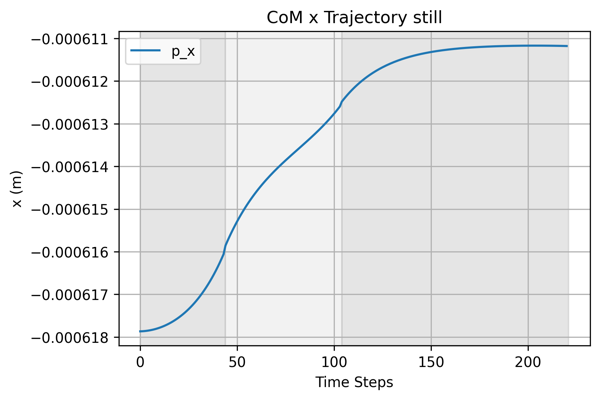
\includegraphics[width=\textwidth]{figures/CoM x Trajectory still.png}
        \caption{Com X Trajectory 1}
        \label{fig:sub1_still}
    \end{subfigure}
    \hfill
    \begin{subfigure}[b]{0.45\textwidth}
        \centering
        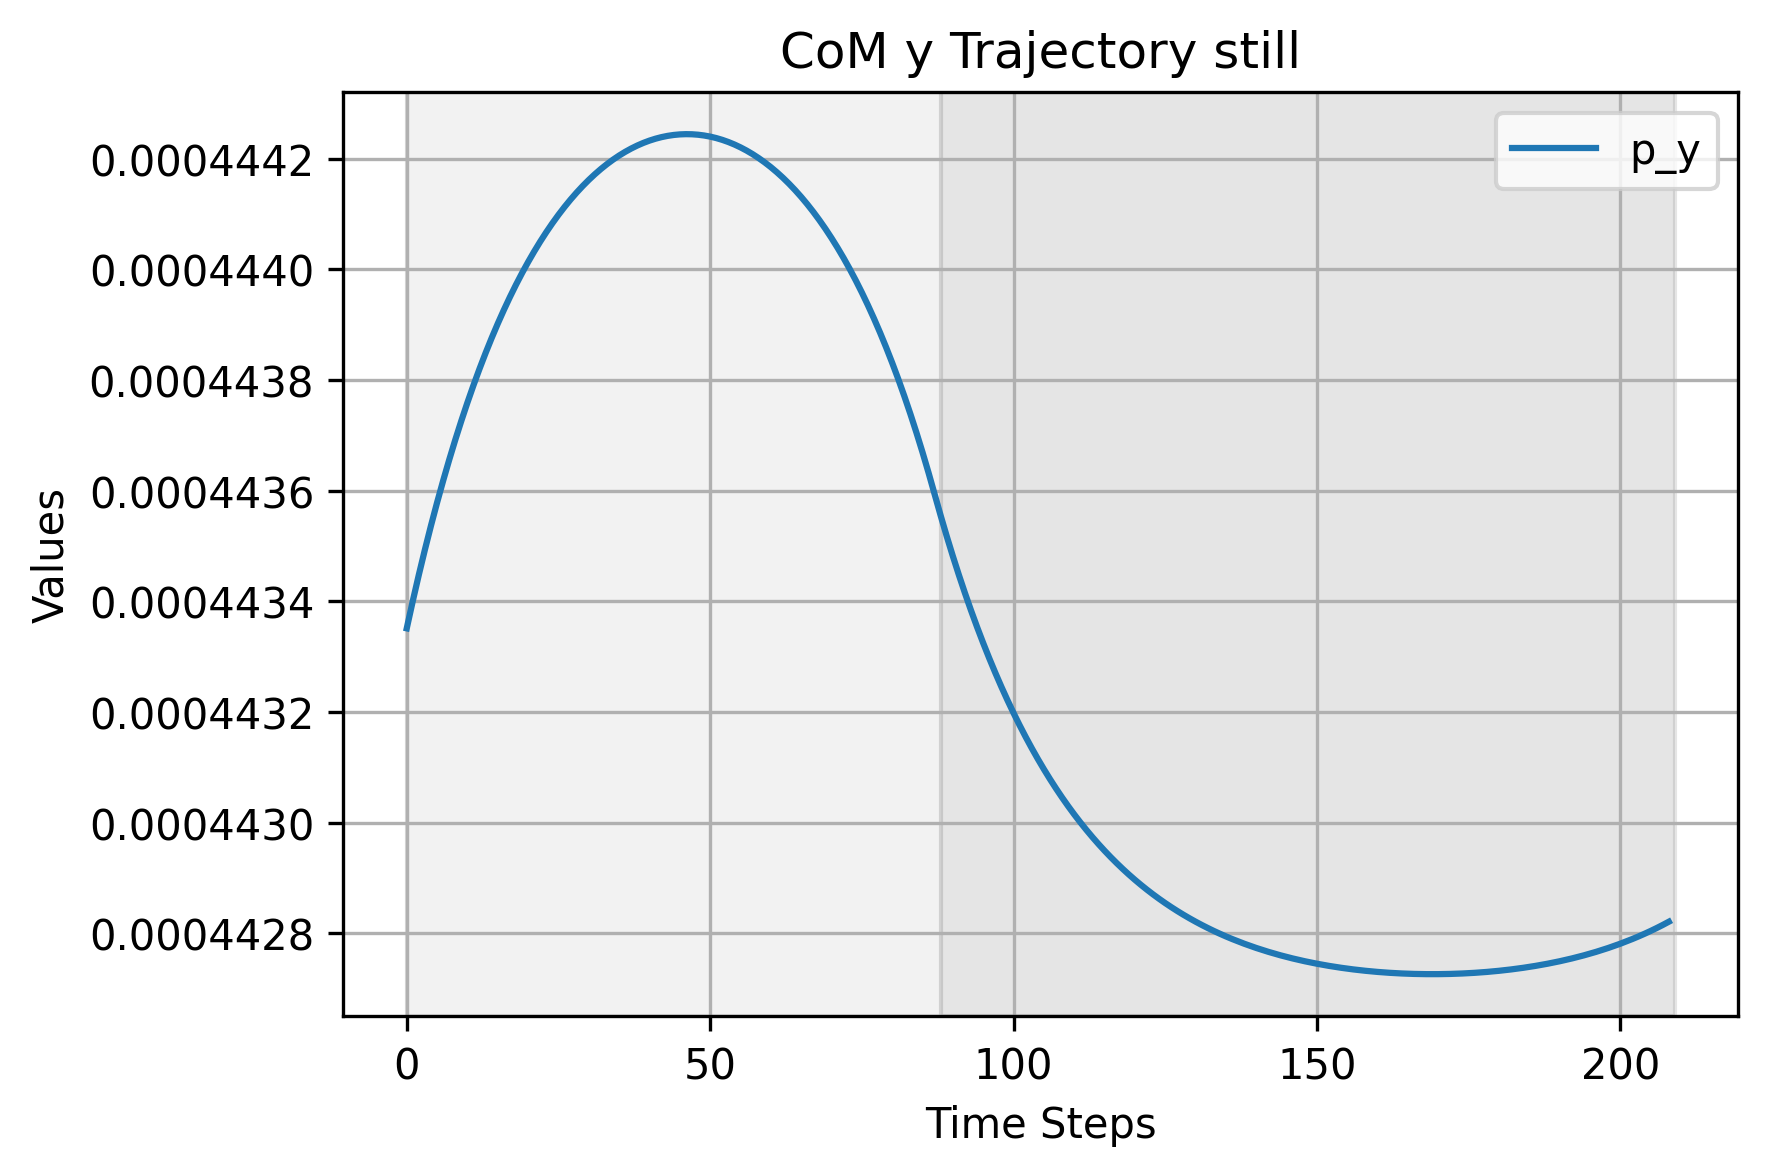
\includegraphics[width=\textwidth]{figures/CoM y Trajectory still.png}
        \caption{Com Y Trajectory 1}
        \label{fig:sub2_still}
    \end{subfigure}
    \hfill
    \begin{subfigure}[b]{0.45\textwidth}
        \centering
        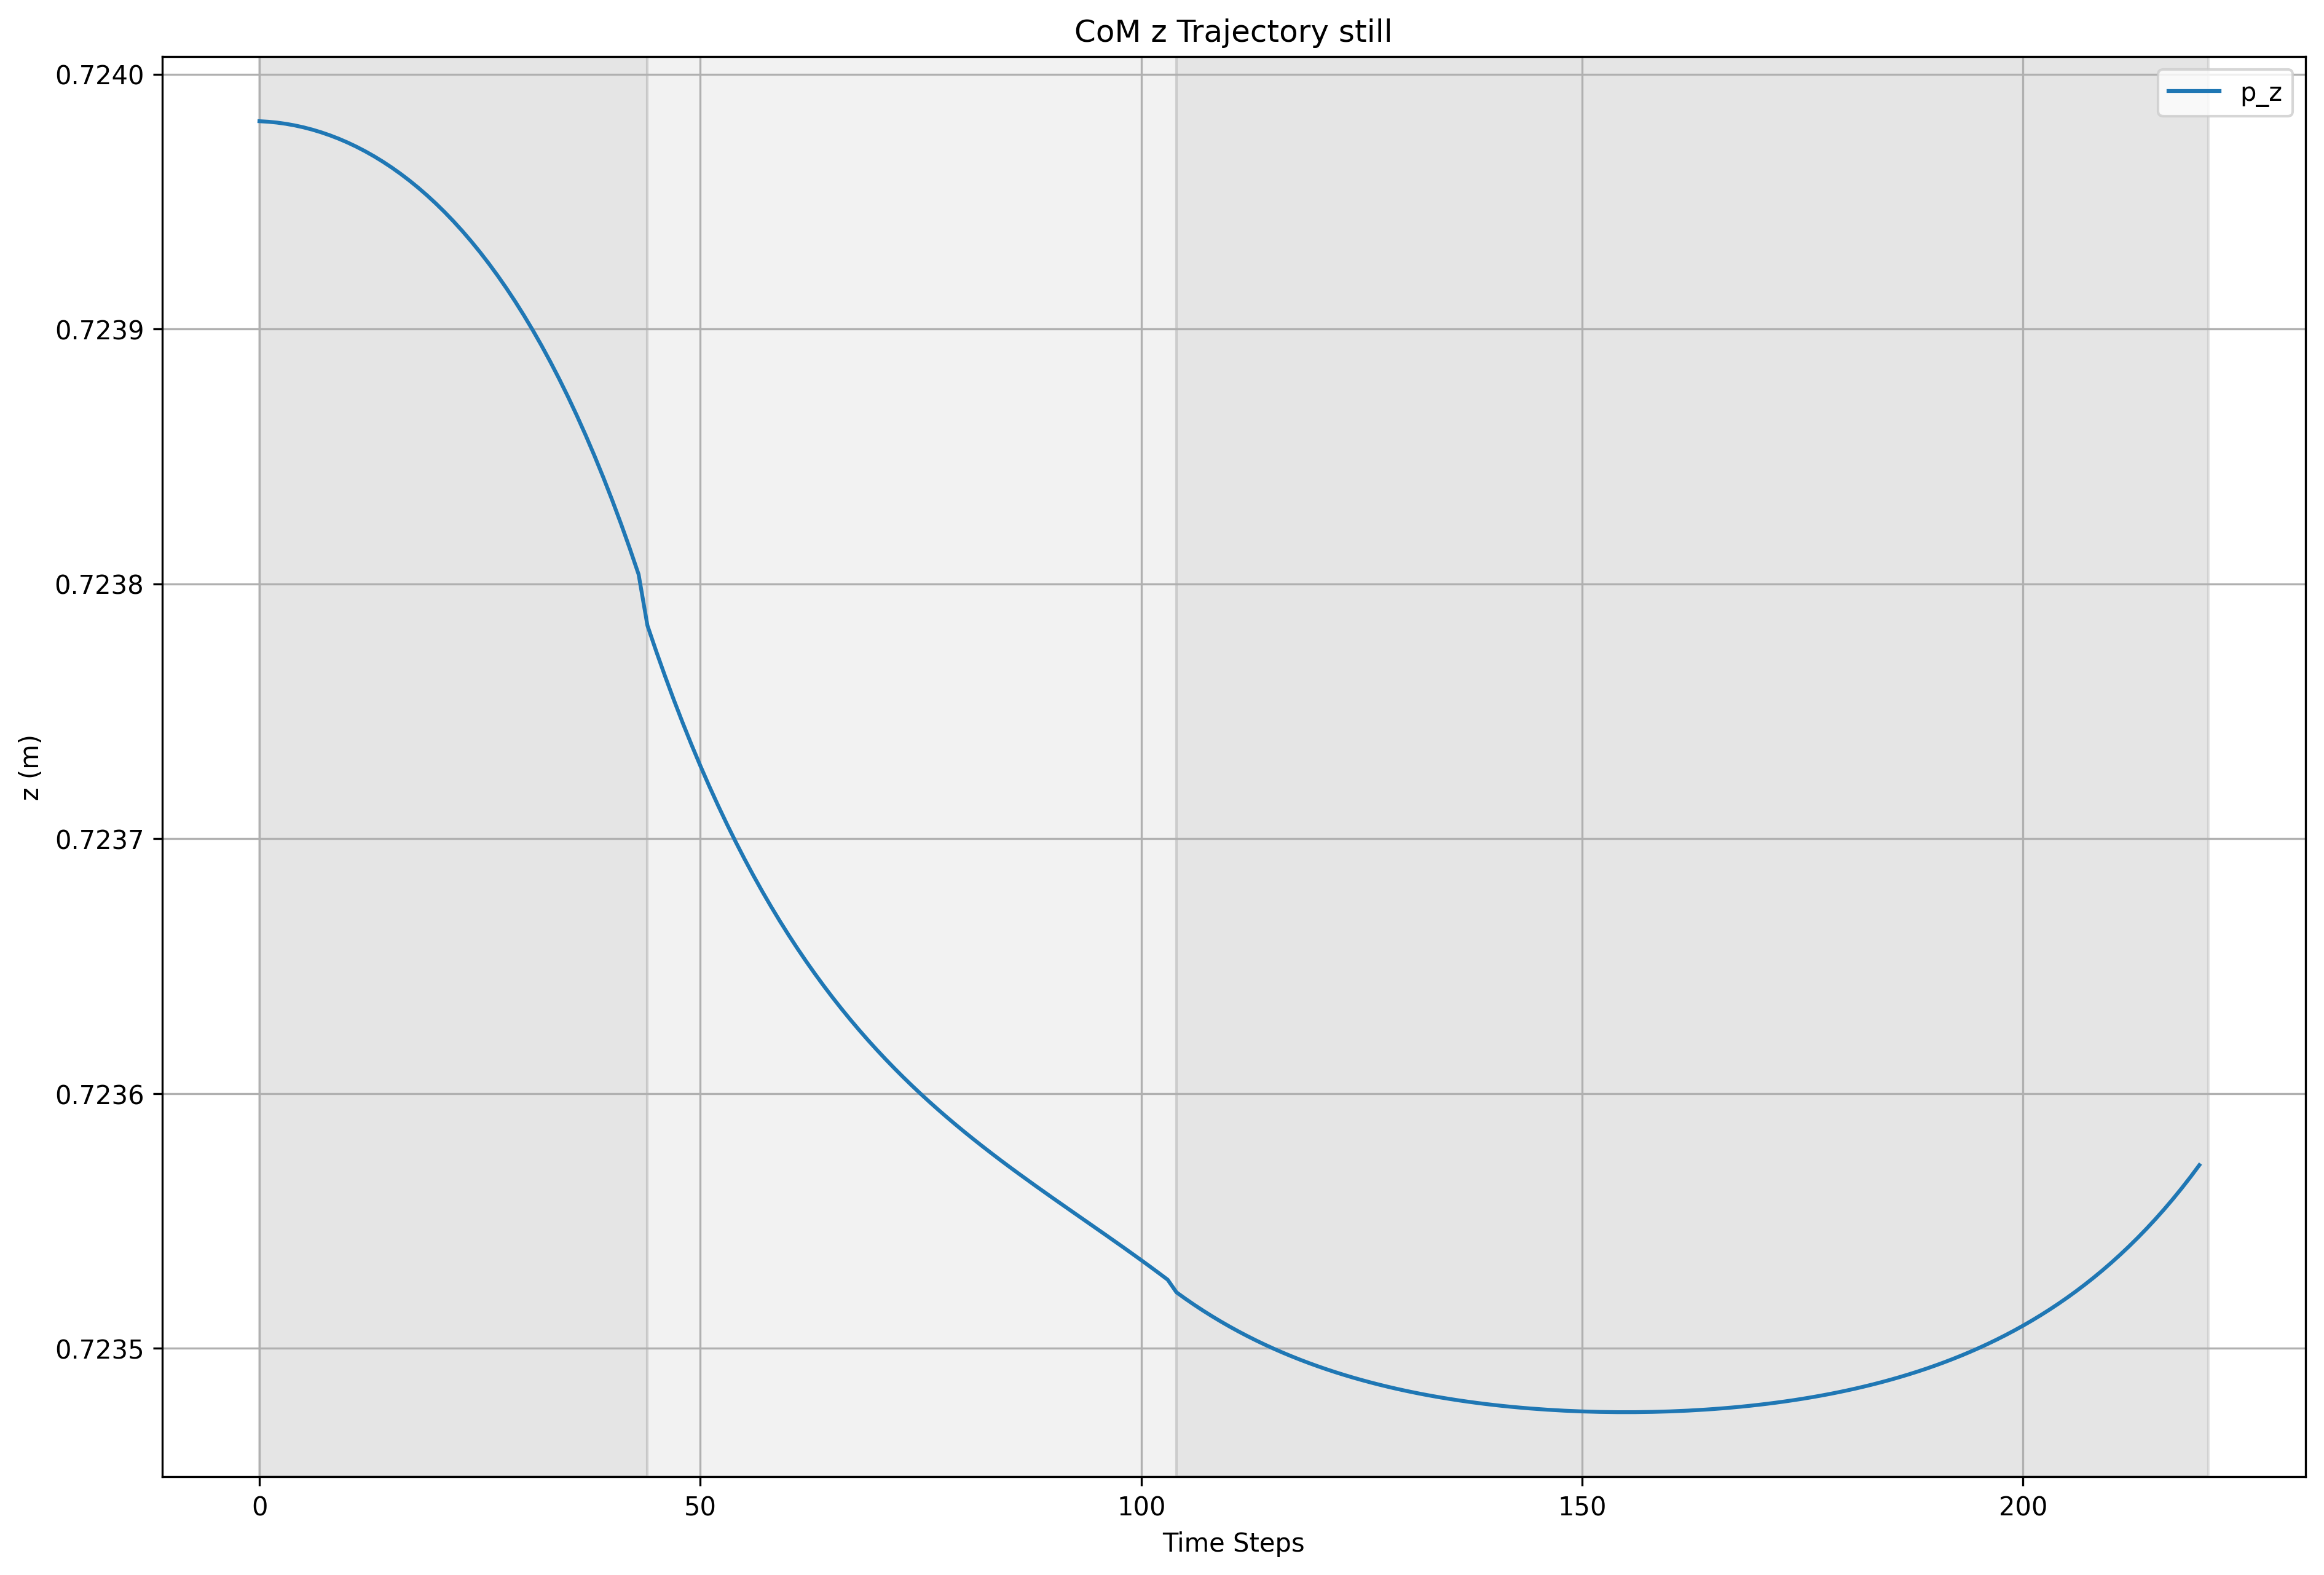
\includegraphics[width=\textwidth]{figures/CoM z Trajectory still.png}
        \caption{Com Z Trajectory 1}
        \label{fig:sub3_still}
    \end{subfigure}
    \caption{Com Trajectory}
    \label{fig:threeimages_still}
\end{figure}

\begin{figure}[htbp]
    \centering
    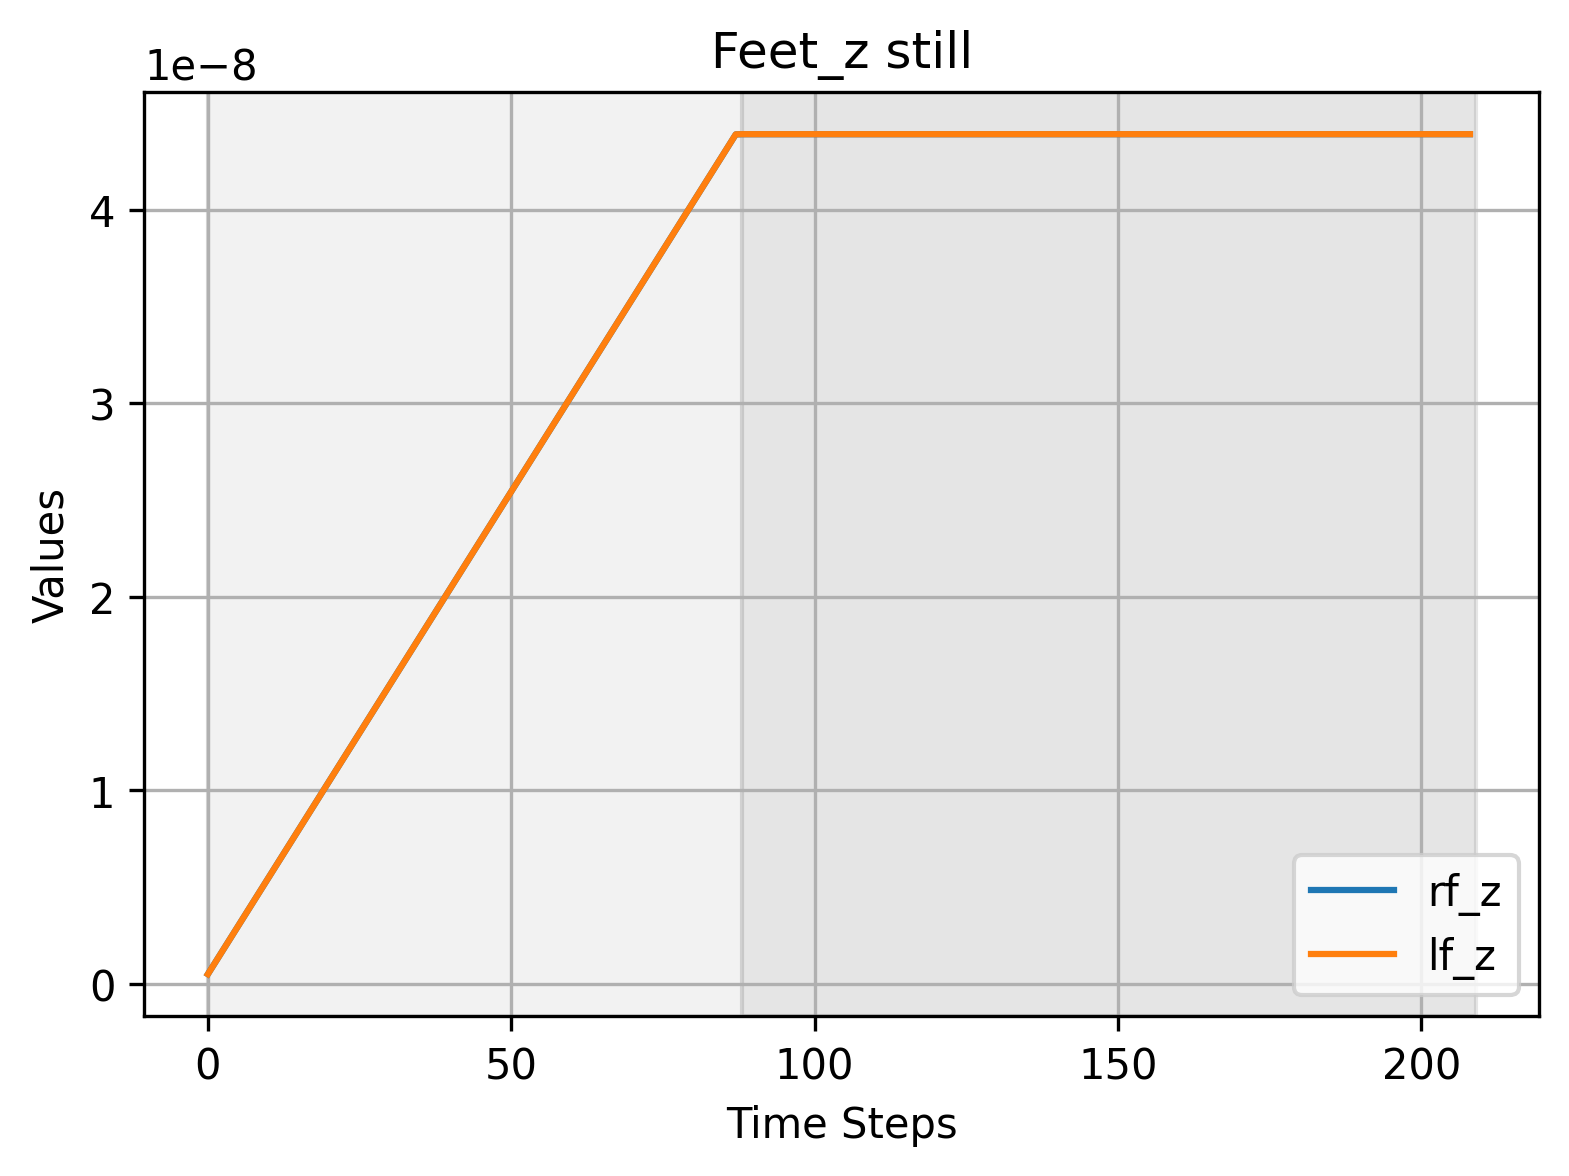
\includegraphics[width=0.6\textwidth]{figures/Feet_z still.png}
    \caption{Feet along Z (scale is 1e-8)}
    \label{fig:feet_still}
\end{figure}


\subsubsection*{State and Input Contact Values}
In the following plots, the main components of the state and input vectors solutions are compared with the reference at each contact step.
\begin{figure}[htbp]
    \centering
    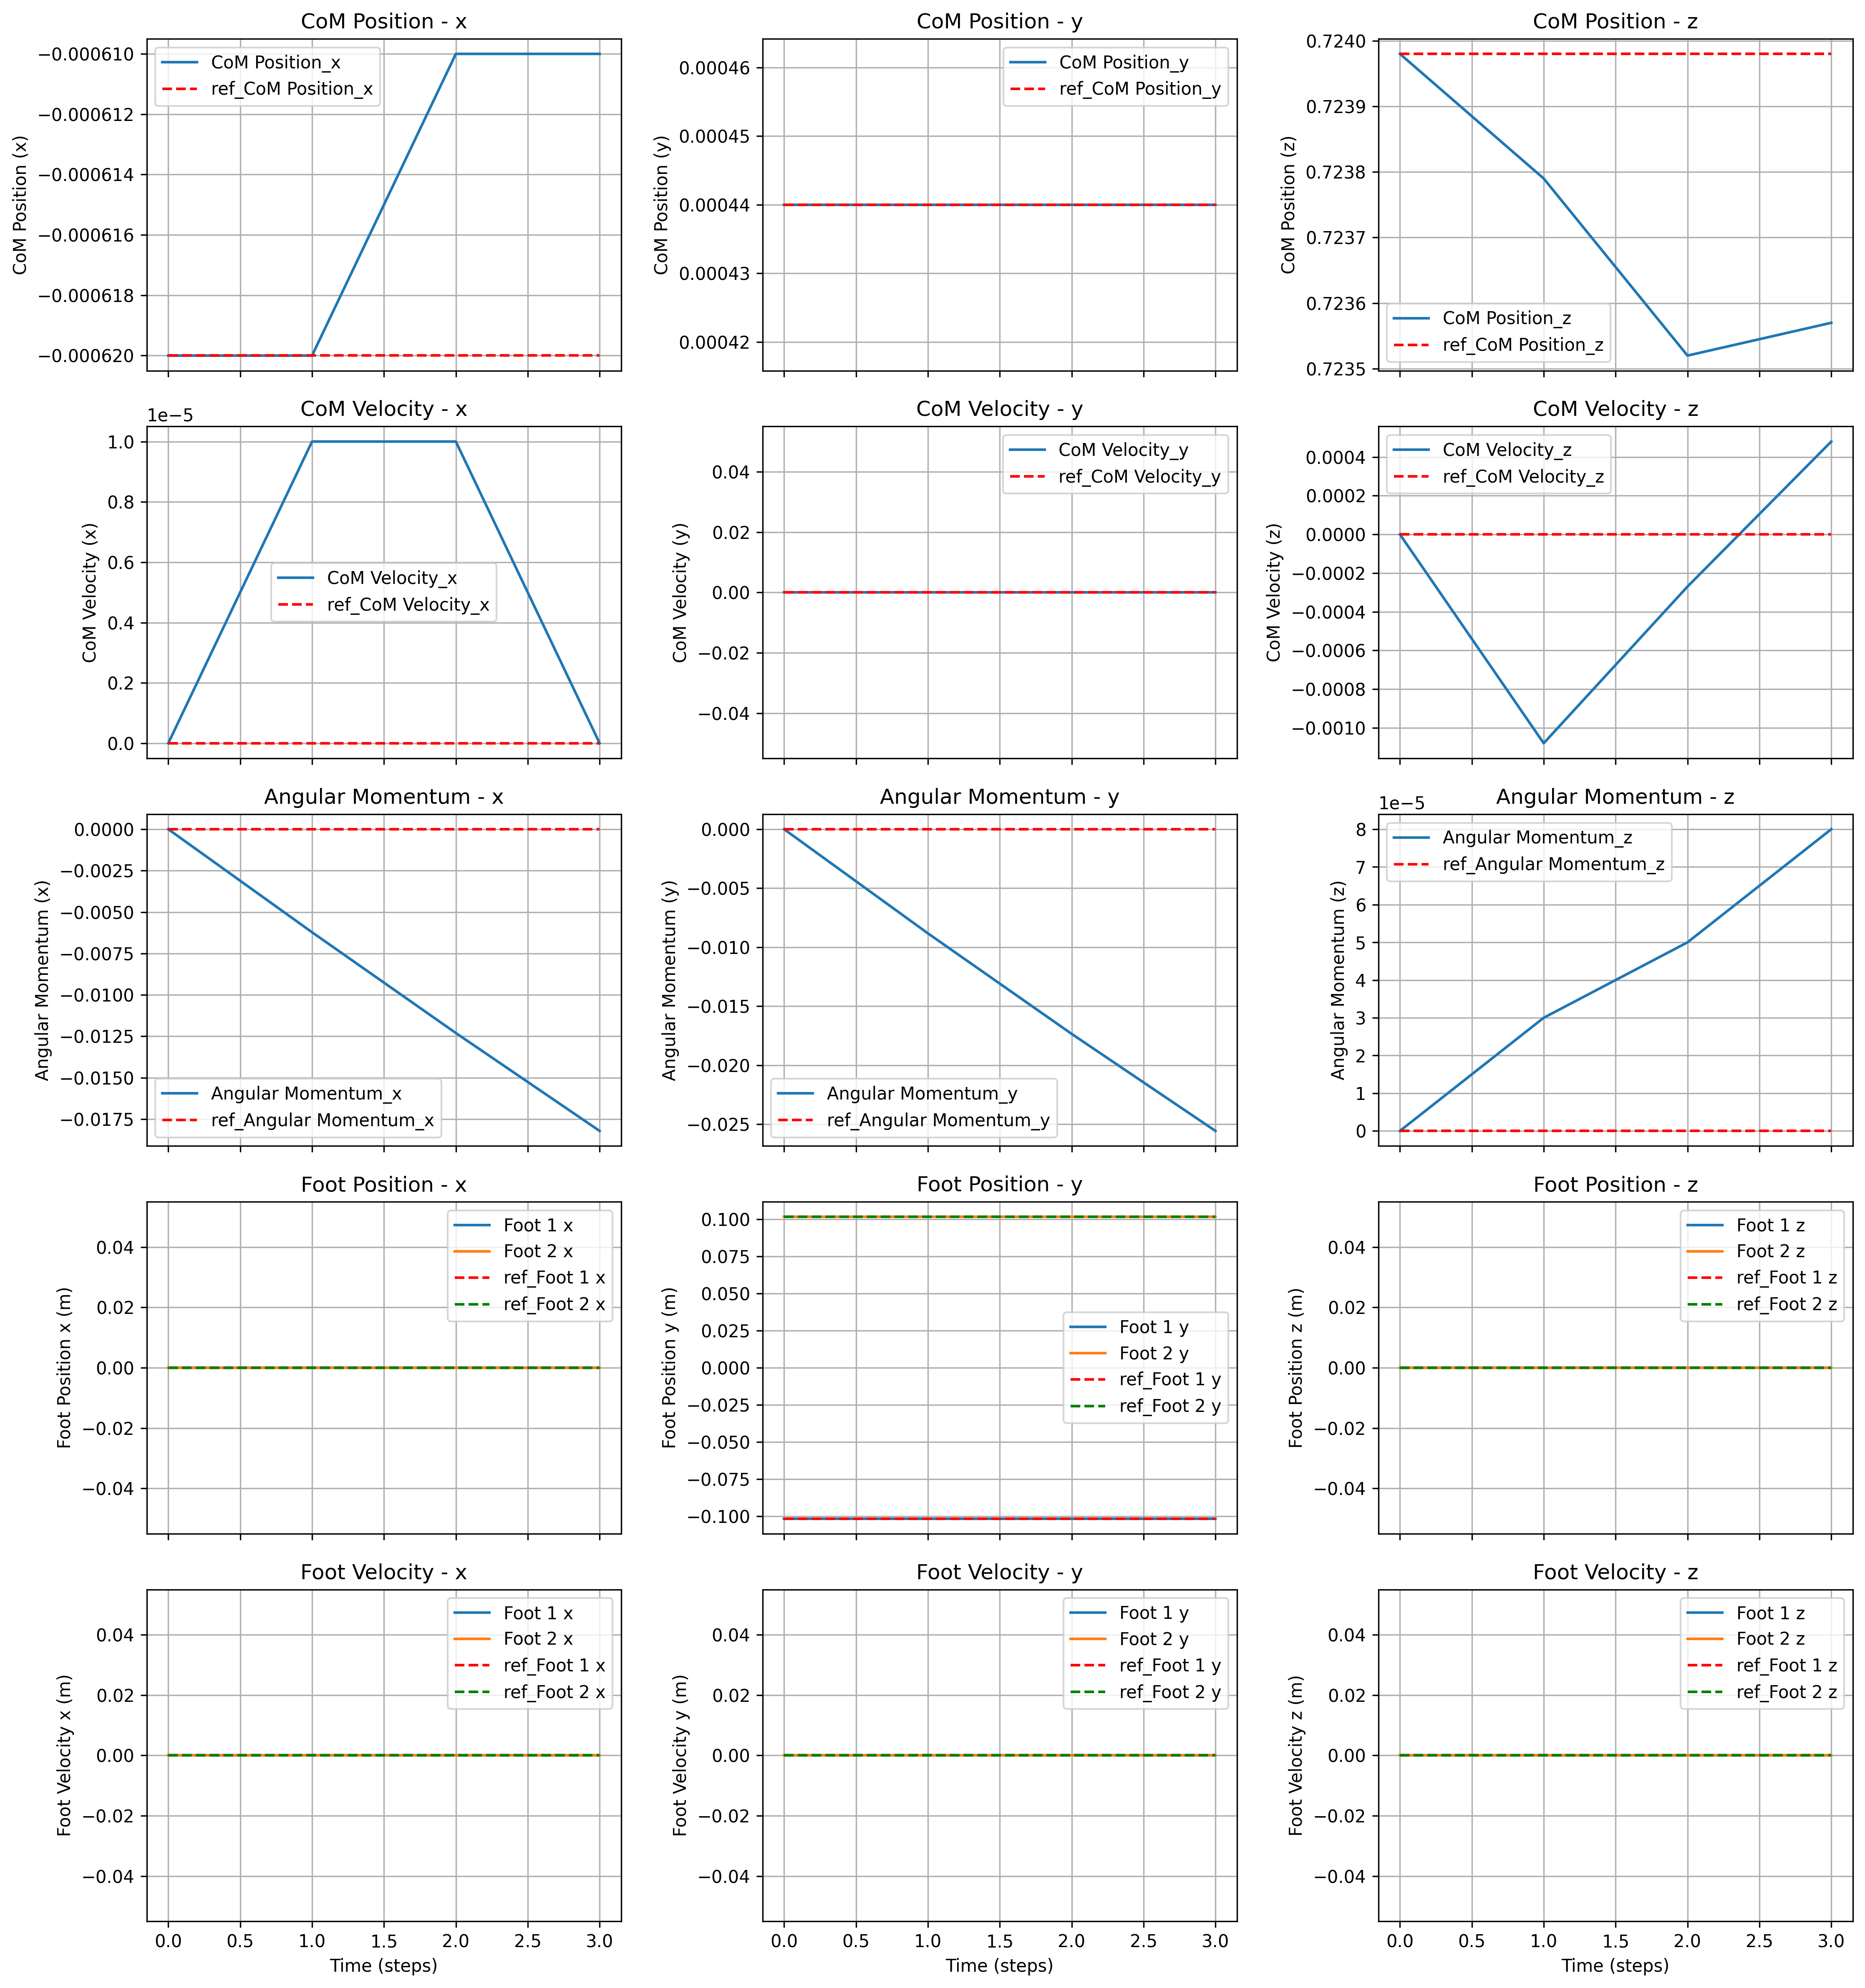
\includegraphics[width=0.6\textwidth]{figures/contact_x_still.png}
    \caption{Trajectory vs Reference: state vector}
    \label{fig:contact_x_still}
\end{figure}

\subsubsection*{Contact Forces}
Another important dynamic aspect pertains to the forces involved. The input vector includes the contact wrench, which describes the mechanical influence that a contact point (such as a foot or hand) exerts on the robot, or vice versa.
In order to satisfy the dynamic balance laws, the environment should exert a reaction force along the Z-axis that is equal to the gravitational force multiplied by the robot's mass. Table \ref{tab:contact_forces_still} below lists the contact forces exerted by the environment on both feet. As shown in the table, when both feet are on the ground, the gravitational force is evenly distributed between the left and right foot.
\begin{table}[H]
\label{tab:contact_forces_still}
\centering
\begin{tabular}{ccc}
\toprule
Right Foot Z & Left Foot Z & $\Sigma_L^k$ \\
\midrule
49.0644 & 49.0531 & [0., 0.] \\
48.8976 & 49.9925 & [0., 0.] \\
48.0847 & 49.0895 & [0., 0.] \\
\bottomrule
\end{tabular}
\caption{Z-axis gravity force and $\Sigma_L^k$ values}
\end{table}

Components of contact wrench, rotational and translational forces, are graphically expressed in the following plots:
\begin{figure}[htbp]
    \centering
    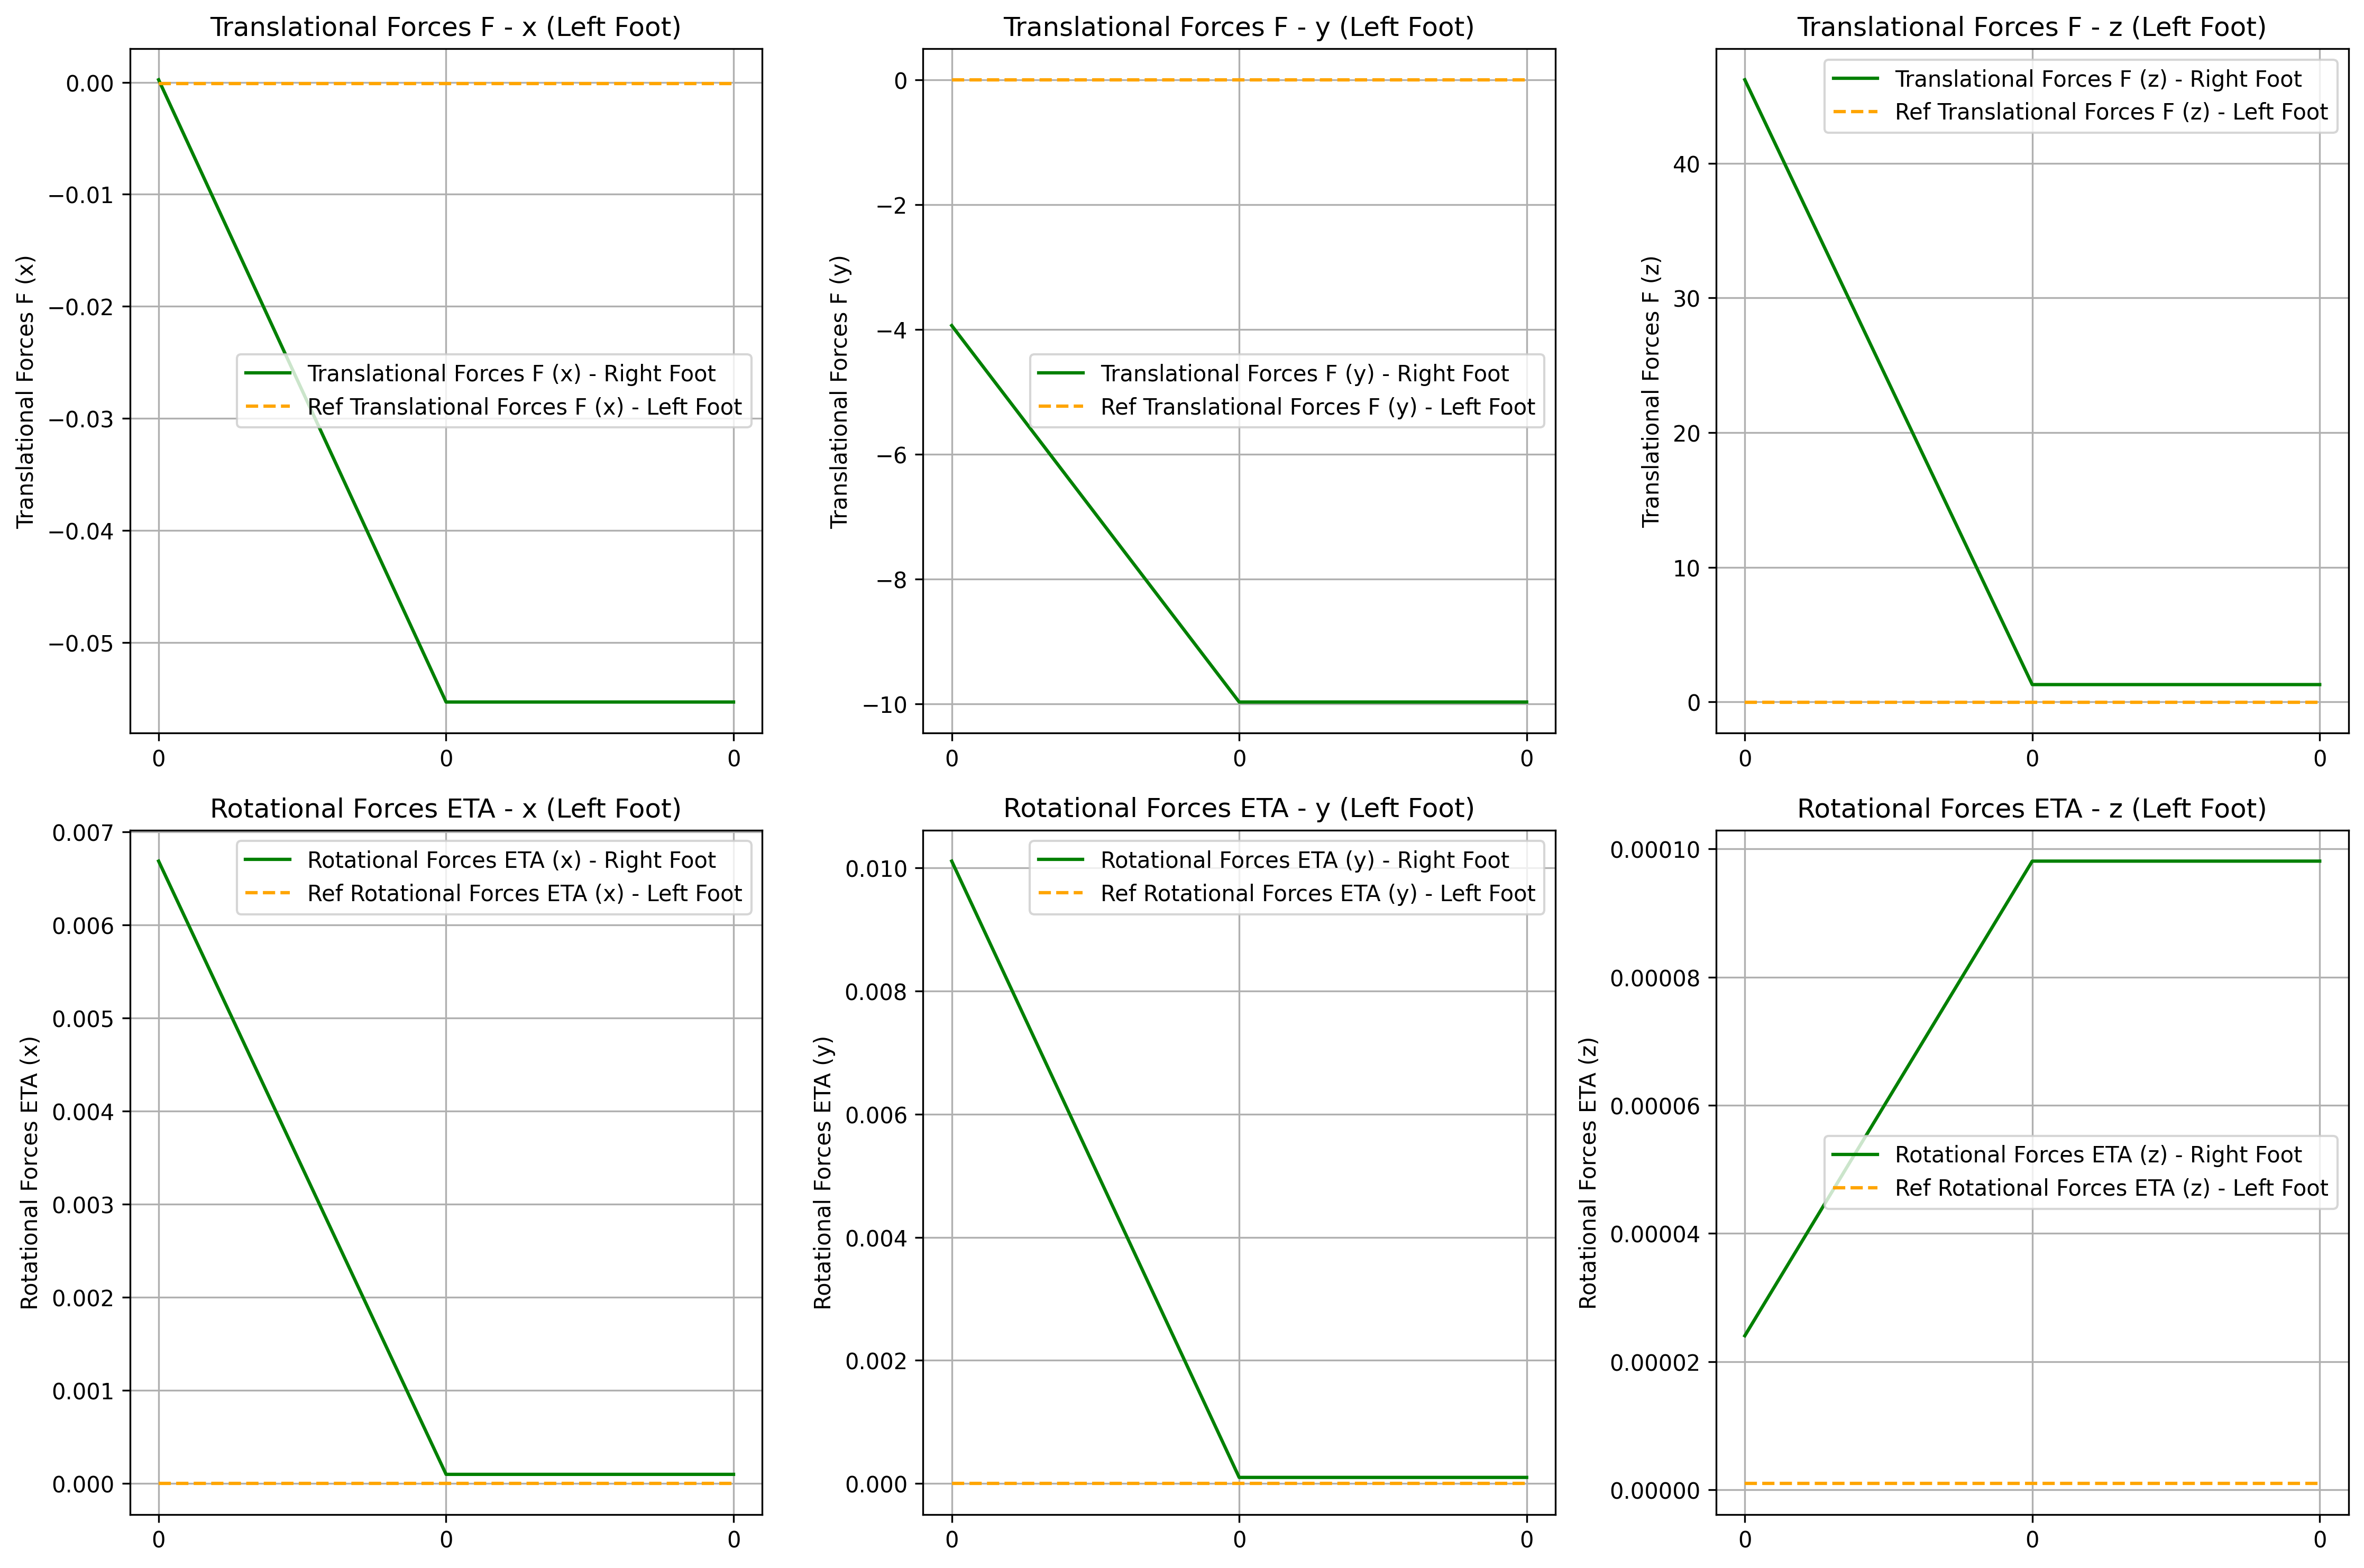
\includegraphics[width=0.8\textwidth]{figures/contact_forces_still.png}
    \caption{Trajectory vs Reference: Forces}
    \label{fig:contact_forces_still}
\end{figure}

\subsection{Walking Task: results}
In this case the state vector has dimension 24 and the input vector has dimension 23.

\subsubsection*{CoM Plots}
The following plots illustrate the trajectory of the Center of Mass (CoM) over time. The alternating light and dark grey backgrounds in the plots indicate the transitions between different phases of the walking motion. As shown in Fig. ~\ref{fig:sub1}, the CoM exhibits linear motion along the x-axis.
In the y-direction, as illustrated in Fig. ~\ref{fig:sub2}, the CoM moves toward the foot that remains on the ground while the other foot is lifted. Specifically, if we consider the first two contact phases: during the first phase, the robot is in double support (both feet on the ground), while in the second phase, the left foot is expected to lift. At the end of the first phase, the CoM has shifted towards the right foot, demonstrating the transition in weight distribution. This pattern of alternating between double and single support phases continues throughout the walking cycle, with the CoM constantly adjusting its position.
In the z-direction, shown in Fig. ~\ref{fig:sub3}, the CoM exhibits a slight up-and-down motion, with a relatively small range of displacement. This vertical motion is consistent with the natural bobbing motion of the body during walking, providing necessary stability and balancing forces. This pattern of CoM movement is crucial for maintaining dynamic stability as the robot progresses through each phase of the gait.
In summary, the CoM trajectory provides key insights into the robot’s walking mechanics, including the shift in weight distribution during transitions between support phases and the vertical adjustments required for balance. These movements are essential for achieving stable locomotion.
\begin{figure}[H]
    \centering
    \begin{subfigure}[b]{0.45\textwidth}
        \centering
        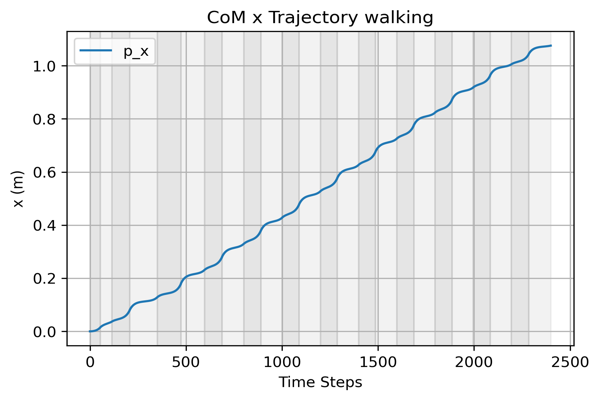
\includegraphics[width=\textwidth]{figures/CoM x Trajectory walking.png}
        \caption{Com X Trajectory 1}
        \label{fig:sub1_walking}
    \end{subfigure}
    \hfill
    \begin{subfigure}[b]{0.45\textwidth}
        \centering
        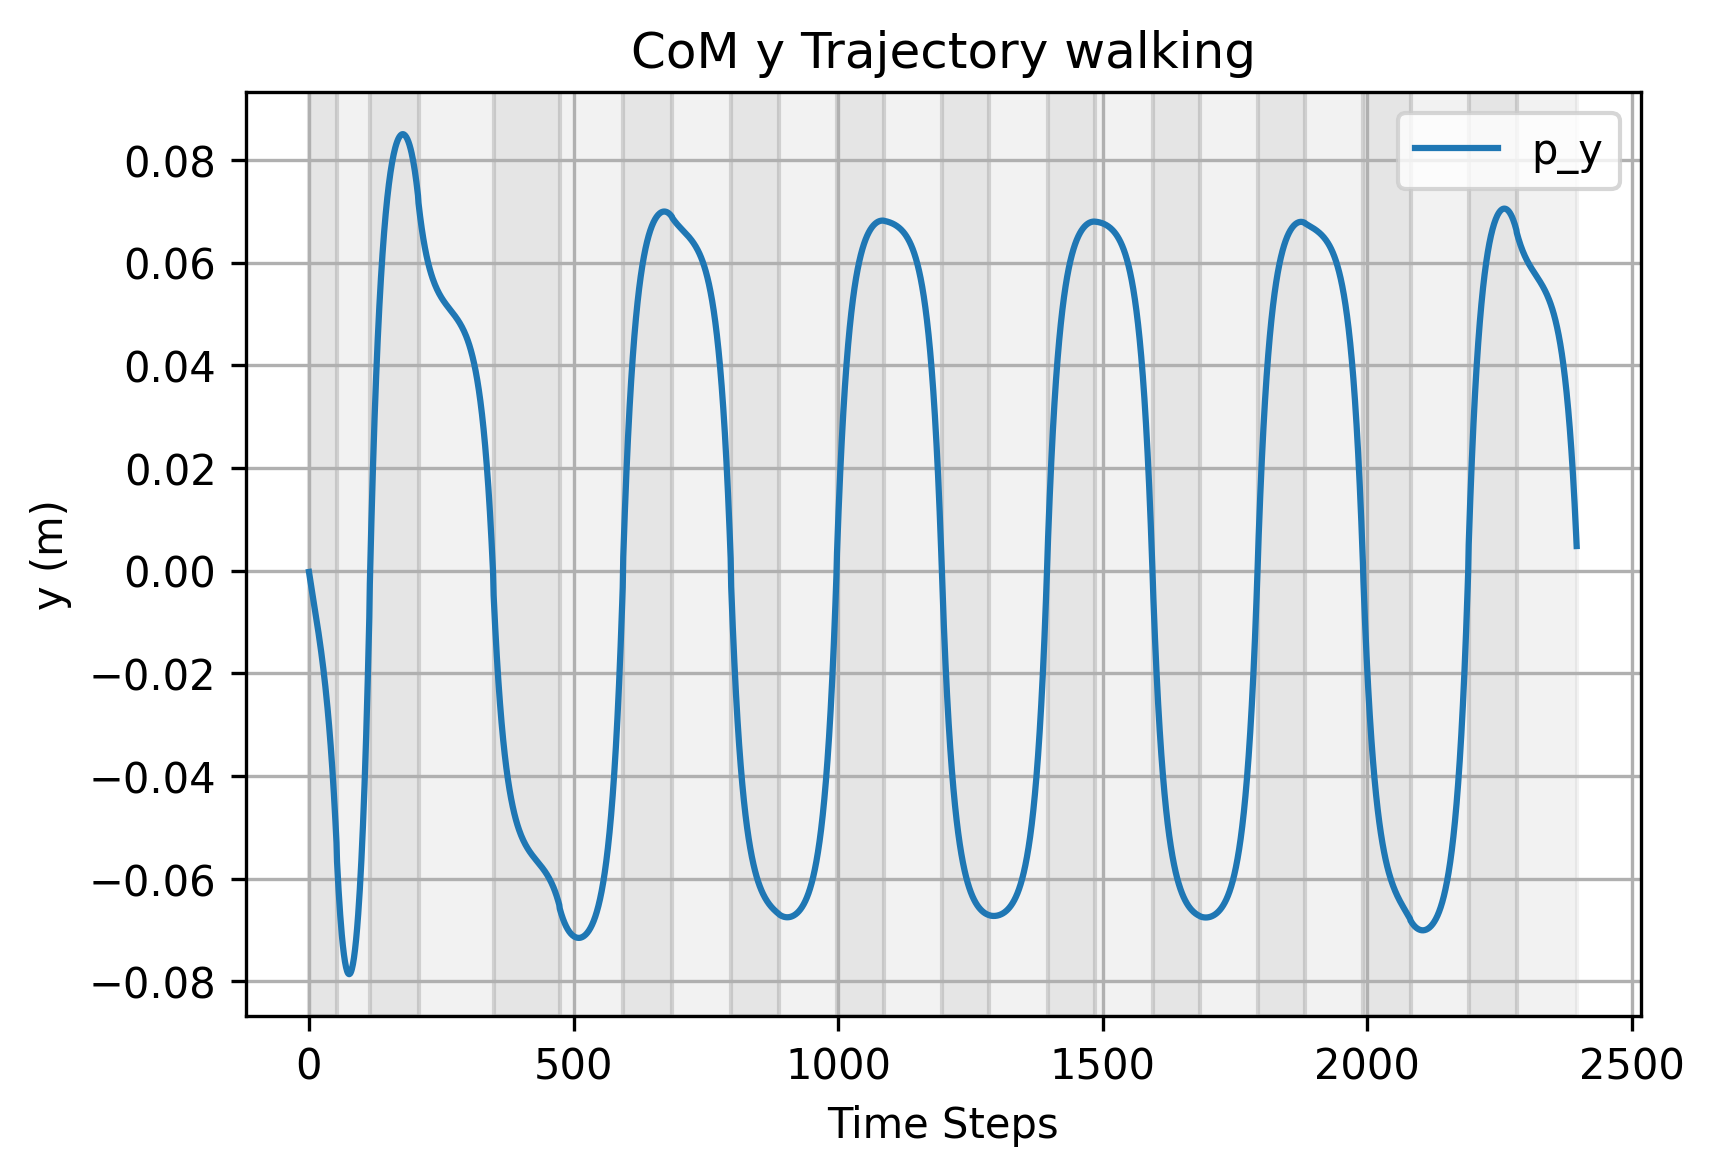
\includegraphics[width=\textwidth]{figures/CoM y Trajectory walking.png}
        \caption{Com Y Trajectory 1}
        \label{fig:sub2_walking}
    \end{subfigure}
    \hfill
    \begin{subfigure}[b]{0.45\textwidth}
        \centering
        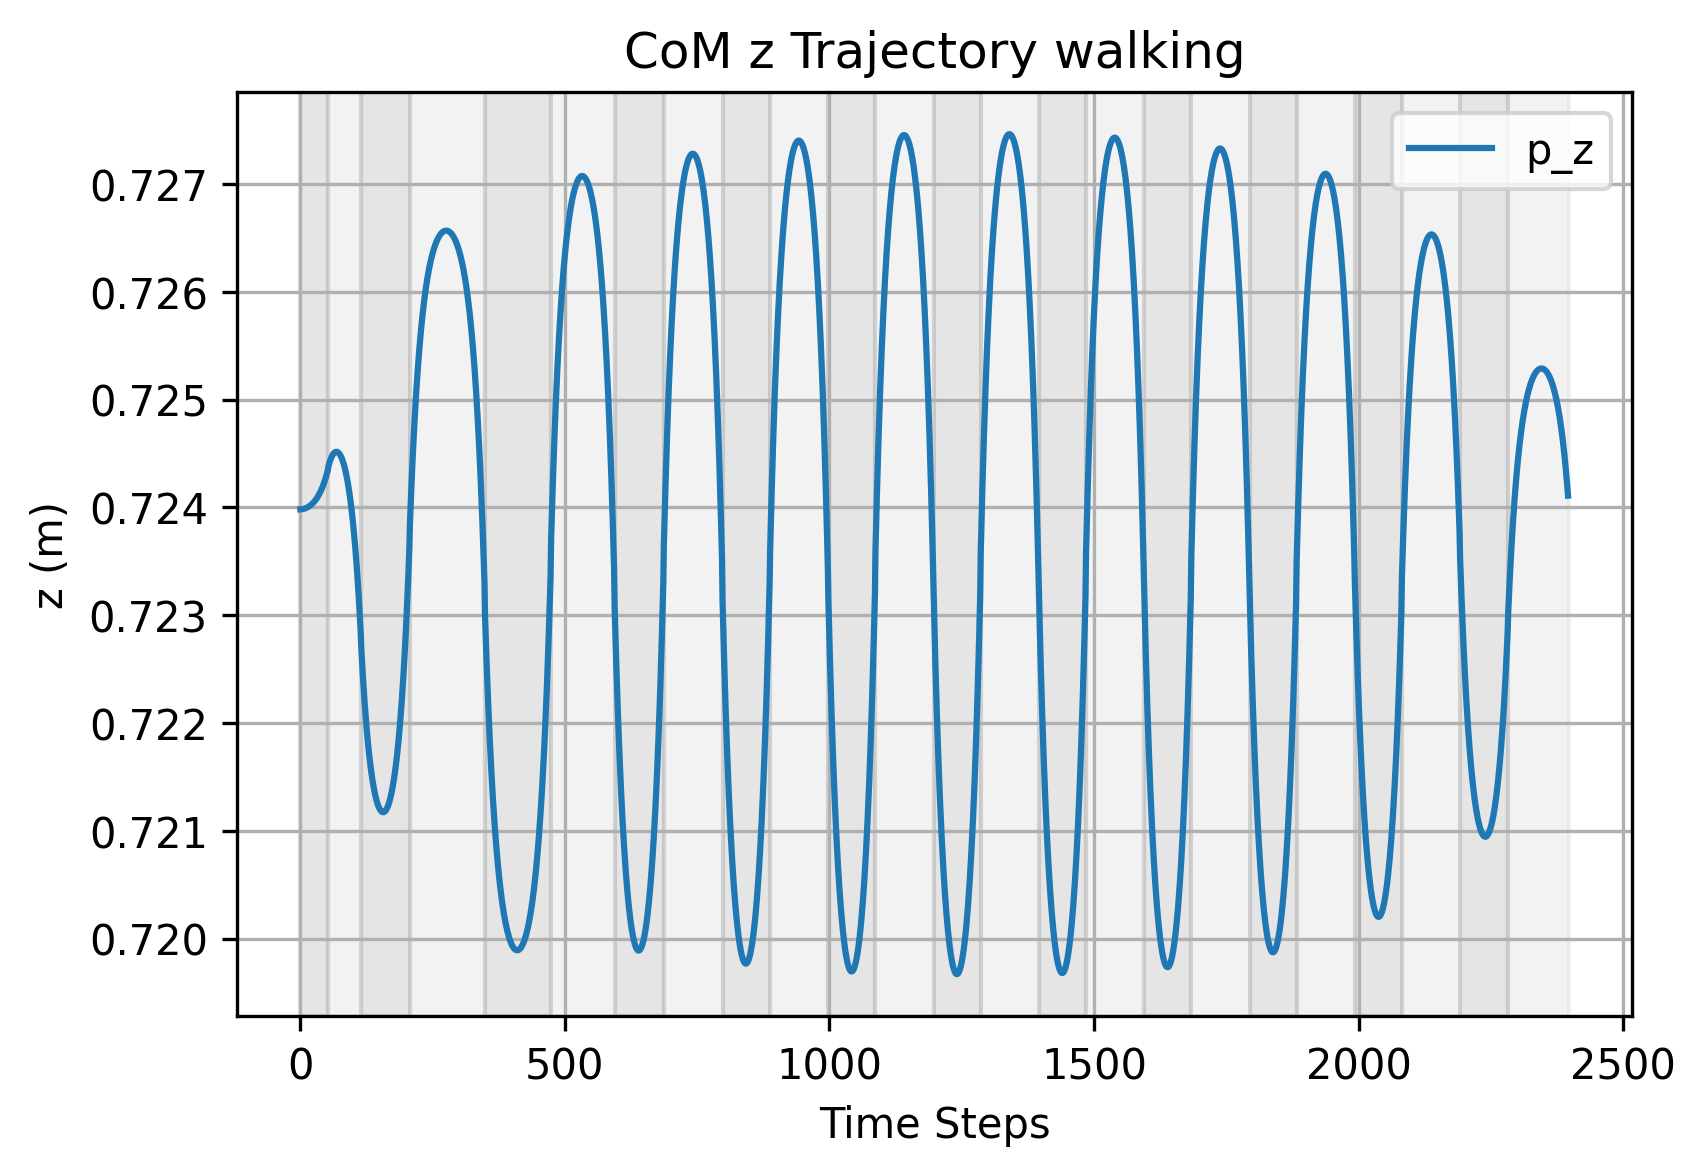
\includegraphics[width=\textwidth]{figures/CoM z Trajectory walking.png}
        \caption{Com Z Trajectory 1}
        \label{fig:sub3_walking}
    \end{subfigure}
    \caption{Com Trajectory}
    \label{fig:threeimages_walking}
\end{figure}
Furthermore, the image below represent the foot position along the Z-axis in time. As one can see, they follow a parabolic profile.  
\begin{figure}[htbp]
    \centering
    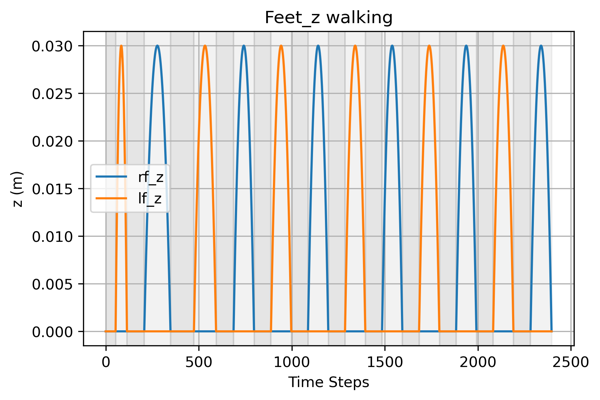
\includegraphics[width=0.6\textwidth]{figures/Feet_z walking.png}
    \caption{Feet along Z}
    \label{fig:feet_walking}
\end{figure}


\subsubsection*{State and Input Contact Values}
As previously said, in the following plots, the main components of the state and input vectors solutions are compared with the reference at each contact step.
\begin{figure}[htbp]
    \centering
    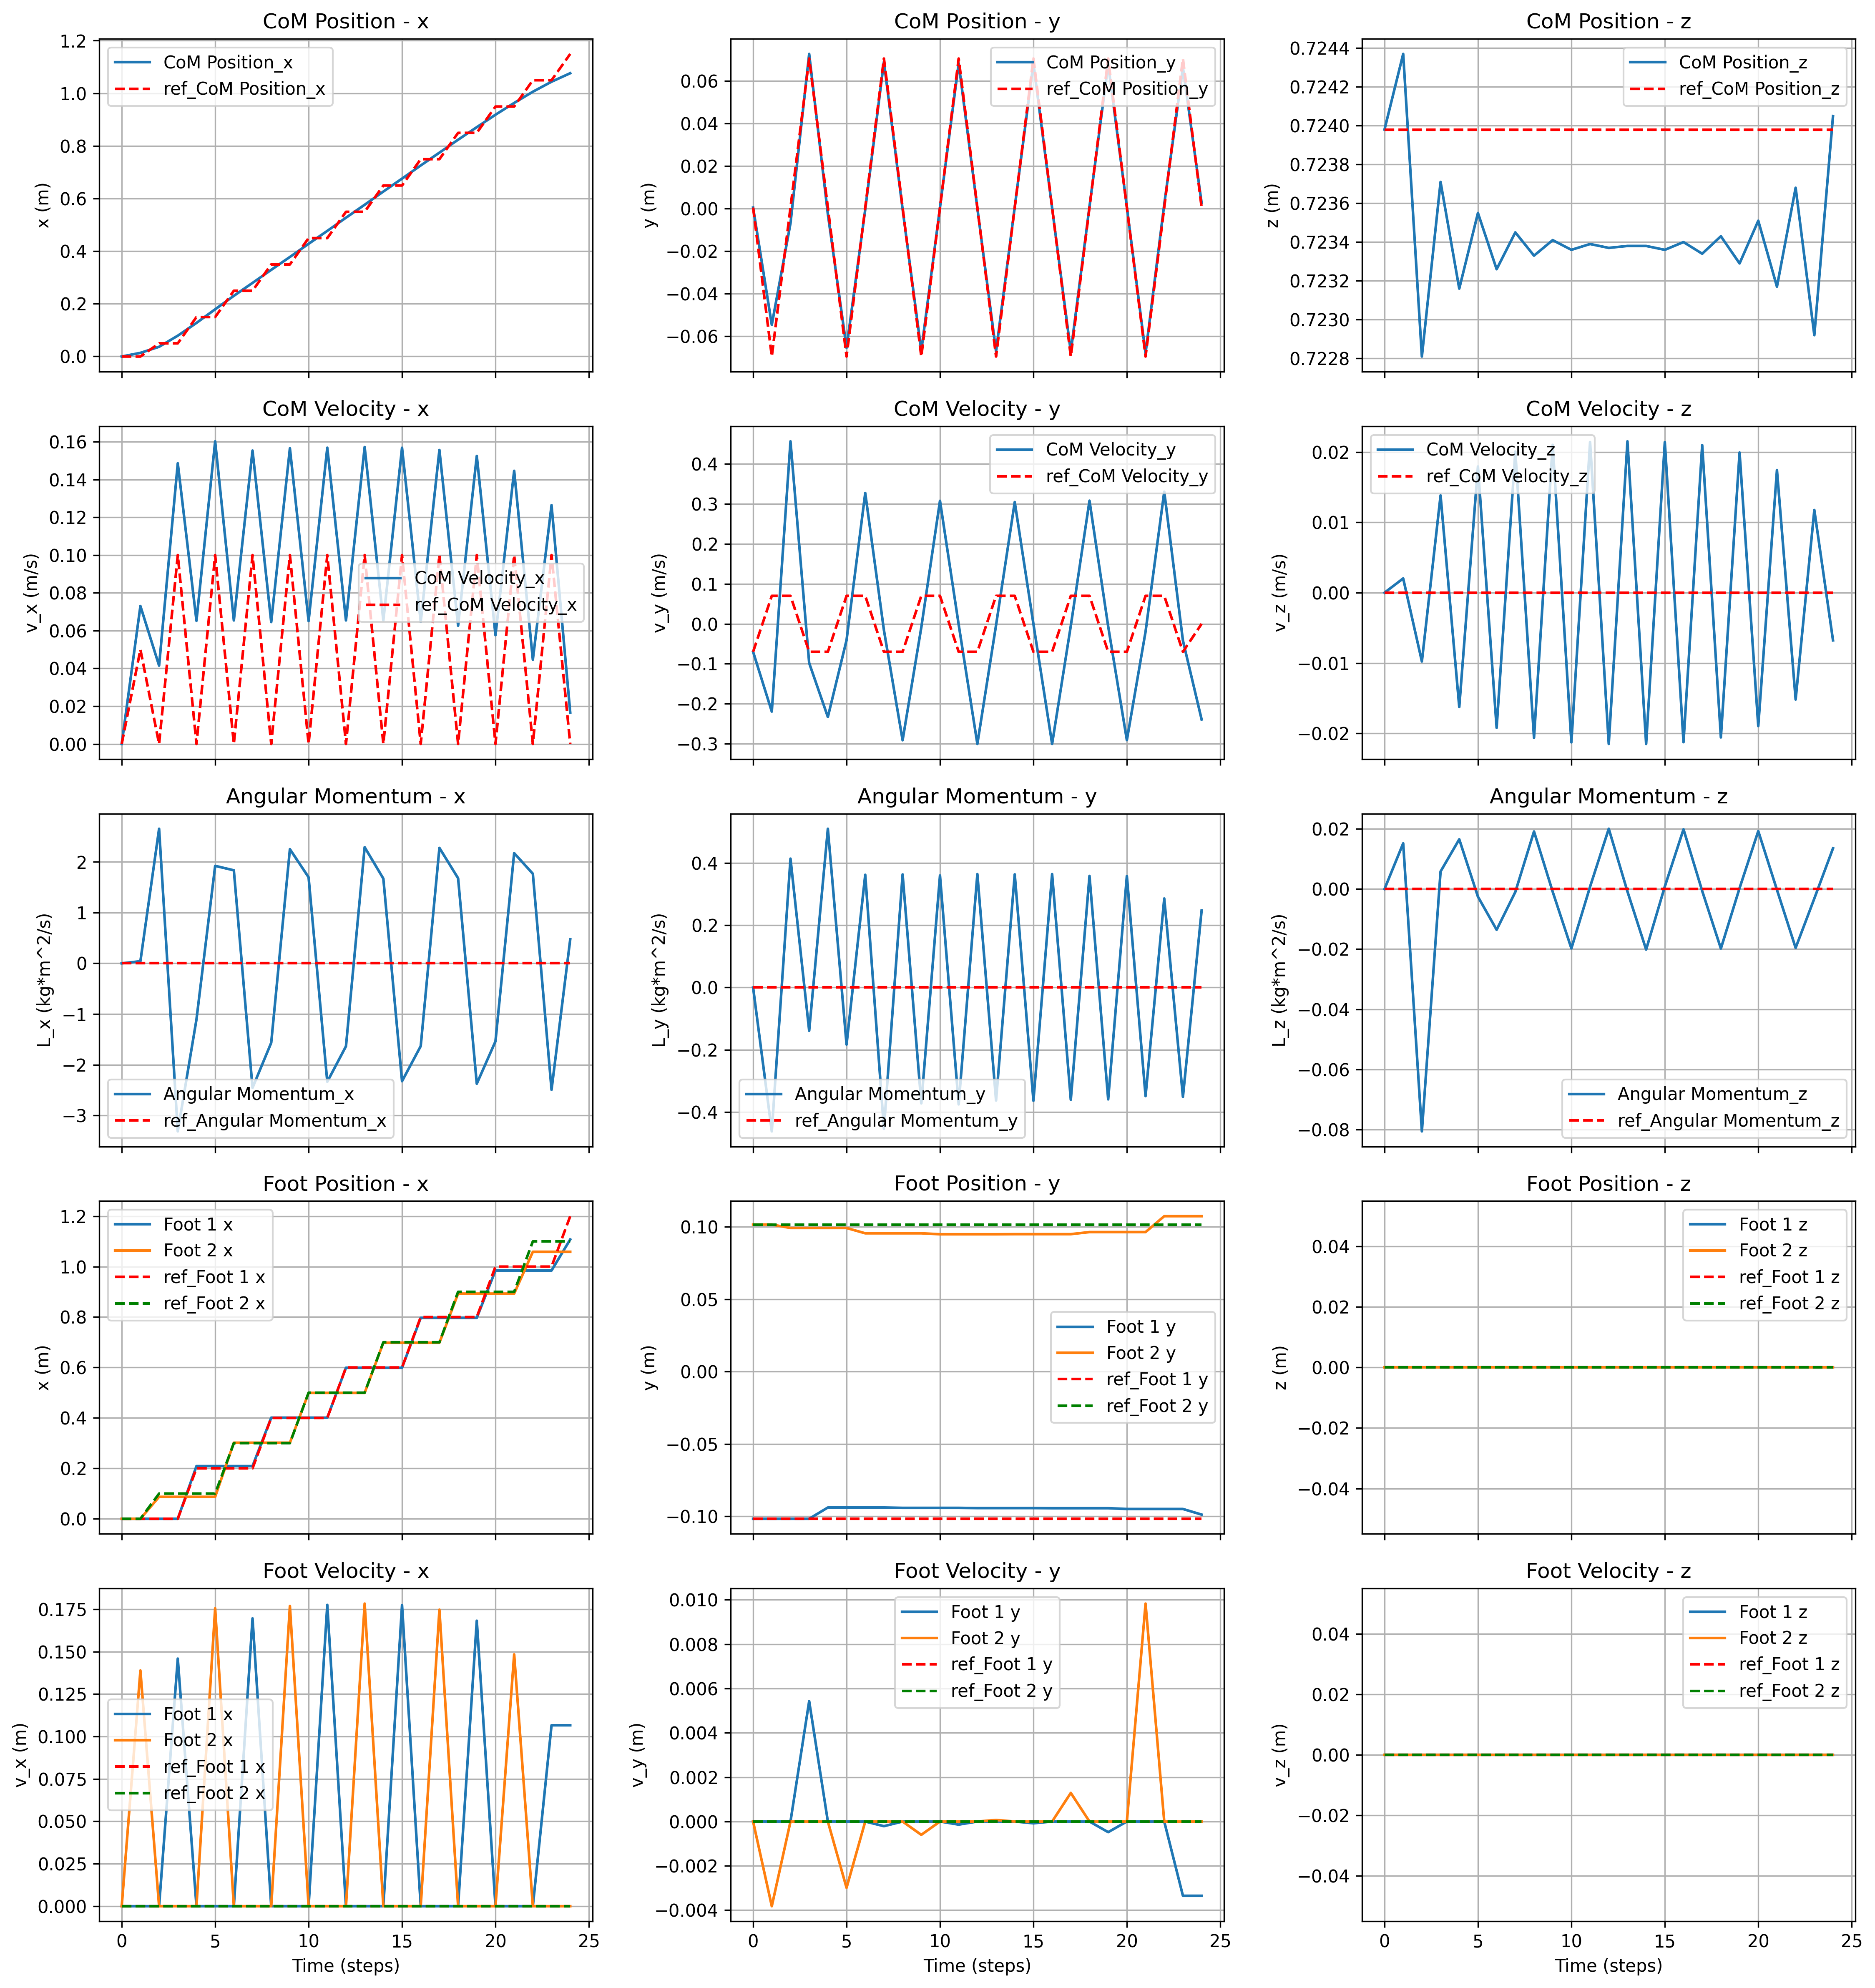
\includegraphics[width=0.6\textwidth]{figures/contact_x_walking.png}
    \caption{Trajectory vs Reference: state vector}
    \label{fig:contact_x_walking}
\end{figure}

\subsubsection*{Contact Forces}
Another key dynamic aspect, which we have already discussed, concerns the forces involved. Specifically, the input vector includes the contact wrench, which captures the mechanical interaction between the robot and contact points, such as the feet or hands. To maintain dynamic balance, the environment must exert a reaction force along the Z-axis equal to the gravitational force, which is the robot's mass multiplied by gravity. Table \ref{tab:contact_forces_walking} below lists the contact forces exerted by the environment on both feet. As shown, when both feet are on the ground, the gravitational force is evenly distributed between the left and right foot, while during single support, the force is applied only to the foot that remains on the ground.\begin{table}[H]
\label{tab:contact_forces_walking}
\centering
\begin{tabular}{ccc}
\toprule
Right Foot Z & Left Foot Z & $\Sigma_L^k$ \\
\midrule
49.0644 & 49.0531 & [0., 0.] \\
97.9551 & 0 & [0., -] \\
48.8973 & 49.65 & [0., 0.] \\
0 & 97.4904 & [-, 0.] \\
49.6528 & 49.1563 & [0., 0.] \\
97.3081 & 0 & [0., -] \\
49.2399 & 49.7241 & [0., 0.] \\
0 & 97.2091 & [-, 0.] \\
49.7388 & 49.293 & [0., 0.] \\
97.1669 & 0 & [0., -] \\
49.3007 & 49.7613 & [0., 0.] \\
0 & 97.1486 & [-, 0.] \\
49.762 & 49.31 & [0., 0.] \\
97.1443 & 0 & [0., -] \\
49.3062 & 49.7655 & [0., 0.] \\
0 & 97.1495 & [-, 0.] \\
49.7557 & 49.3045 & [0., 0.] \\
97.1685 & 0 & [0., -] \\
49.2815 & 49.7467 & [0., 0.] \\
0 & 97.216 & [-, 0.] \\
49.7003 & 49.254 & [0., 0.] \\
97.3264 & 0 & [0., -] \\
49.1286 & 49.6485 & [0., 0.] \\
0 & 97.5828 & [-, 0.] \\
\bottomrule
\end{tabular}
\caption{Z-axis gravity force and $\Sigma_L^k$ values}
\end{table}

Again, components of contact wrench, rotational and translational forces, are graphically expressed in the following plots:
\begin{figure}[htbp]
    \centering
    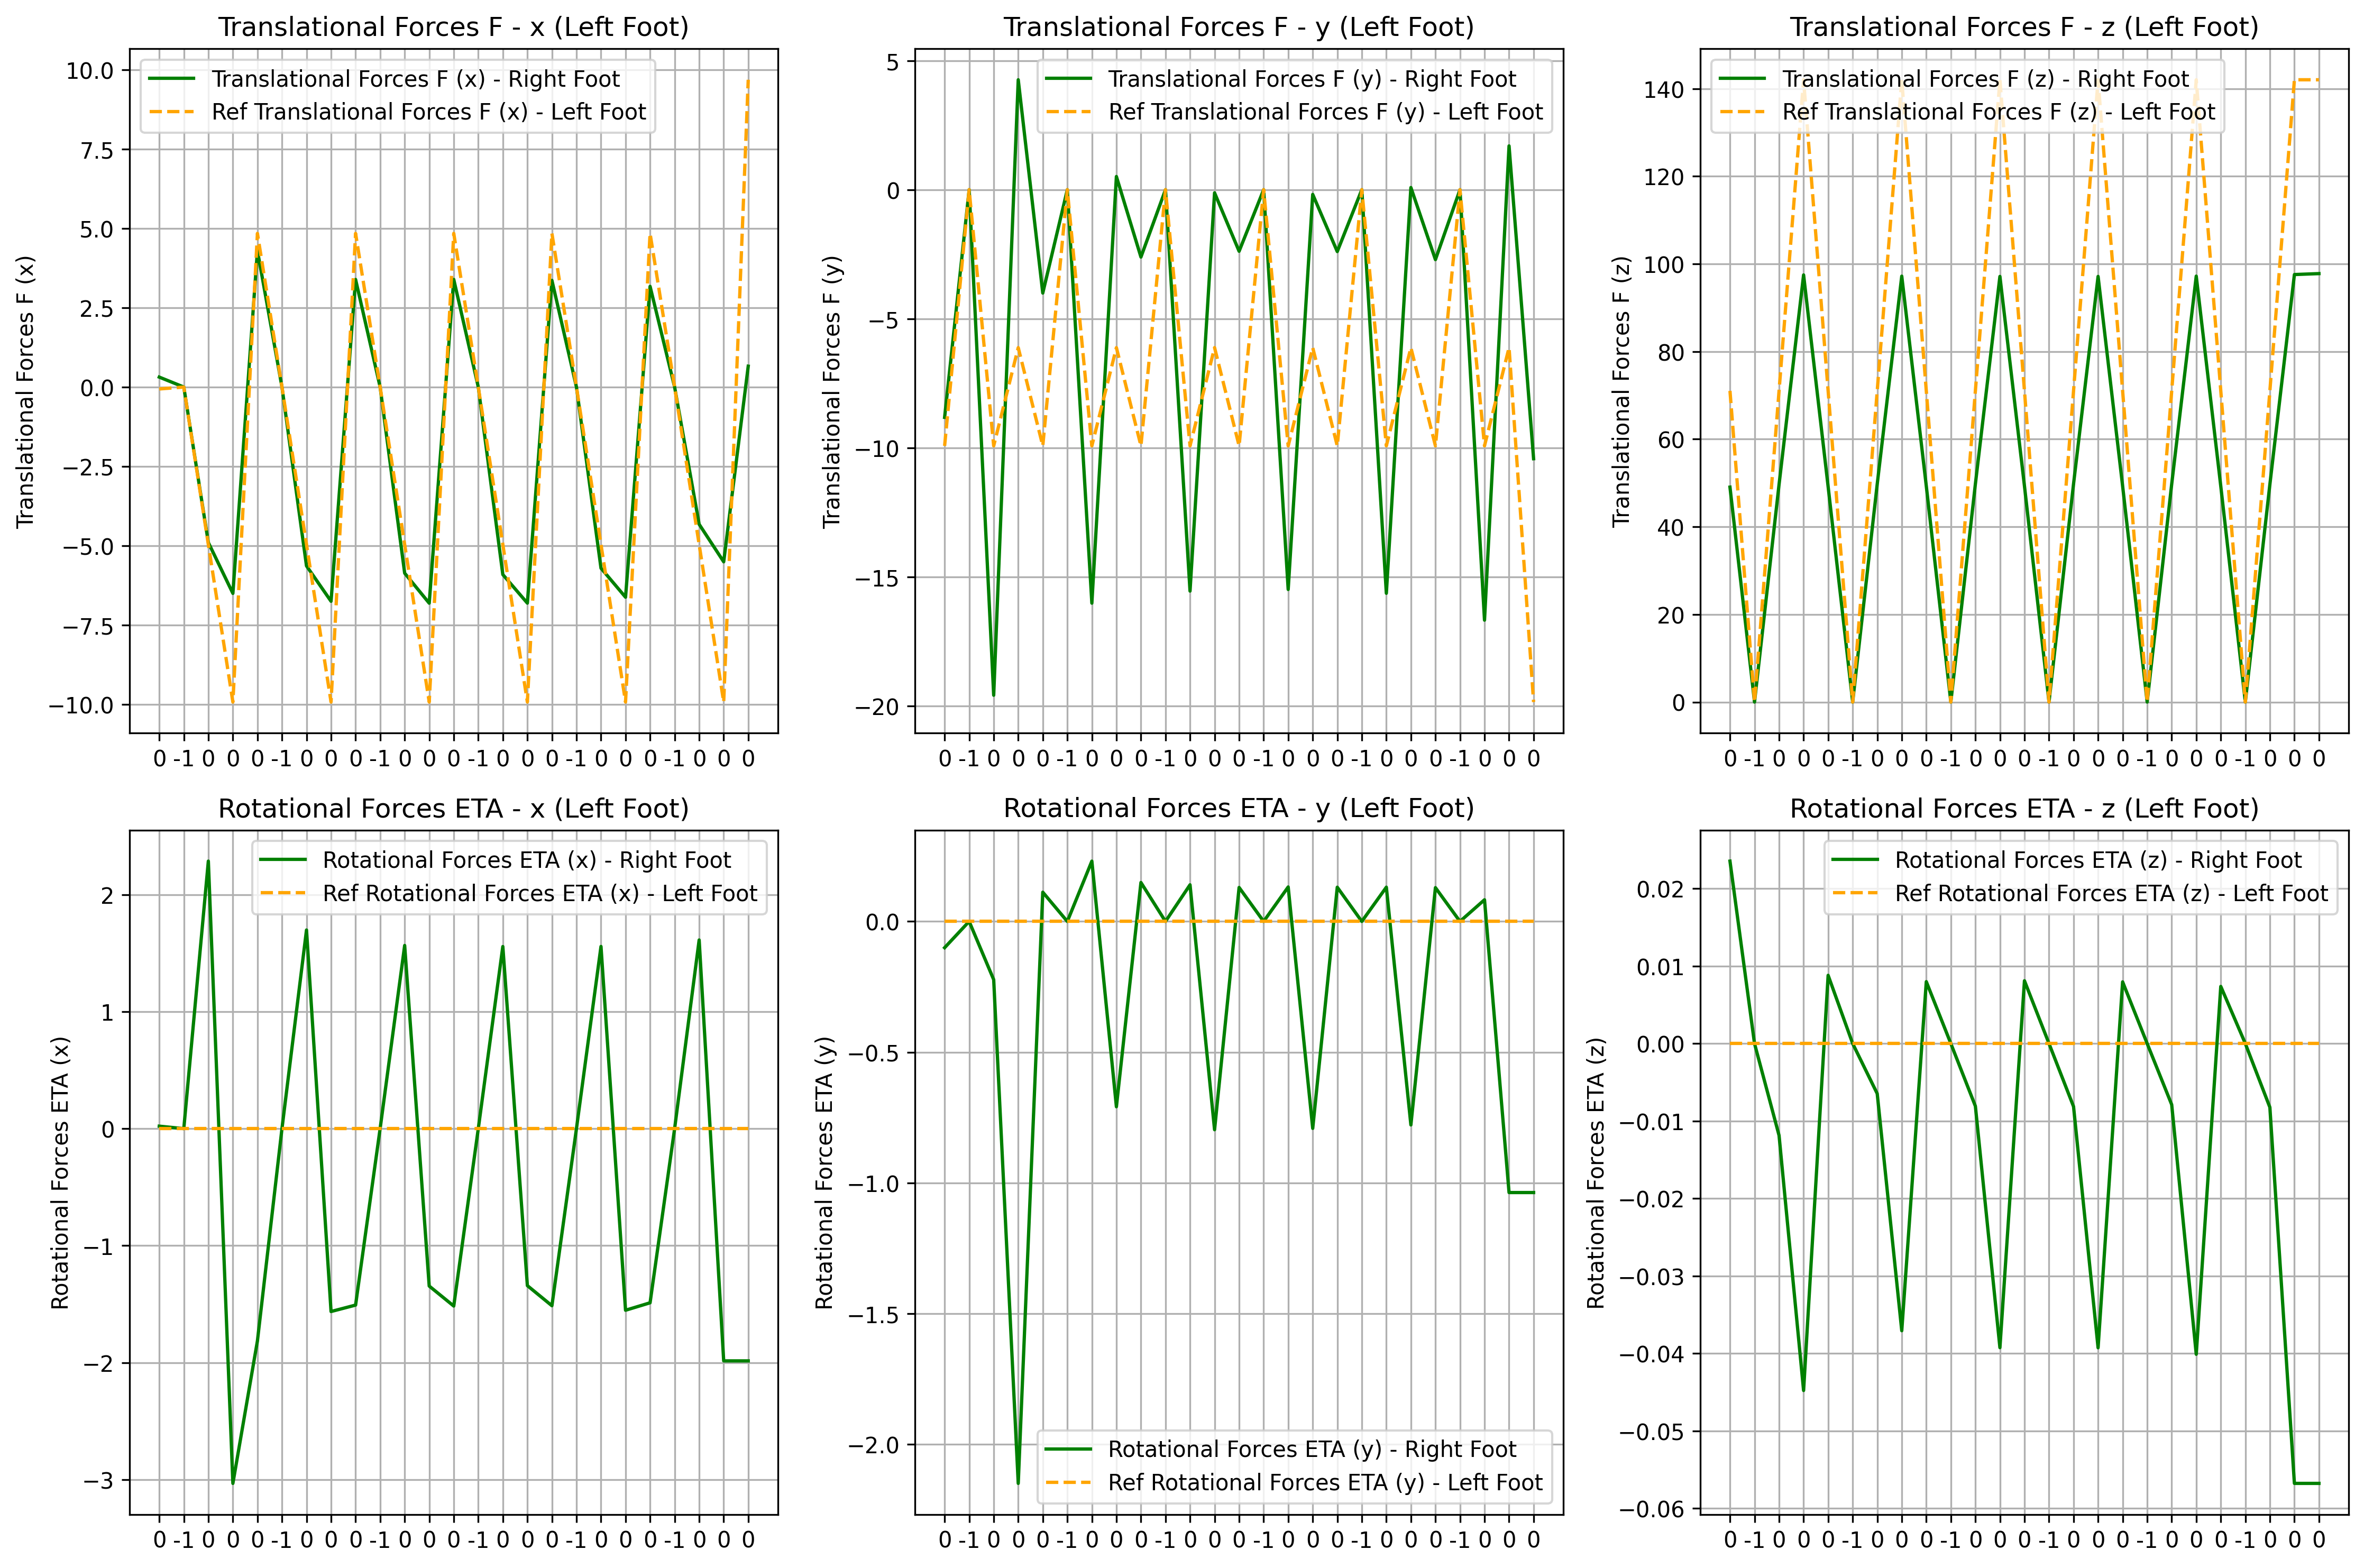
\includegraphics[width=0.8\textwidth]{figures/contact_forces_walking.png}
    \caption{Trajectory vs Reference: Forces}
    \label{fig:contact_forces_walking}
\end{figure}

\newpage
\subsubsection*{Robot representation}
In this section it is possible to visualize the path followed by the CoM, right and left foot in time:
\begin{figure}[htbp]
    \centering
    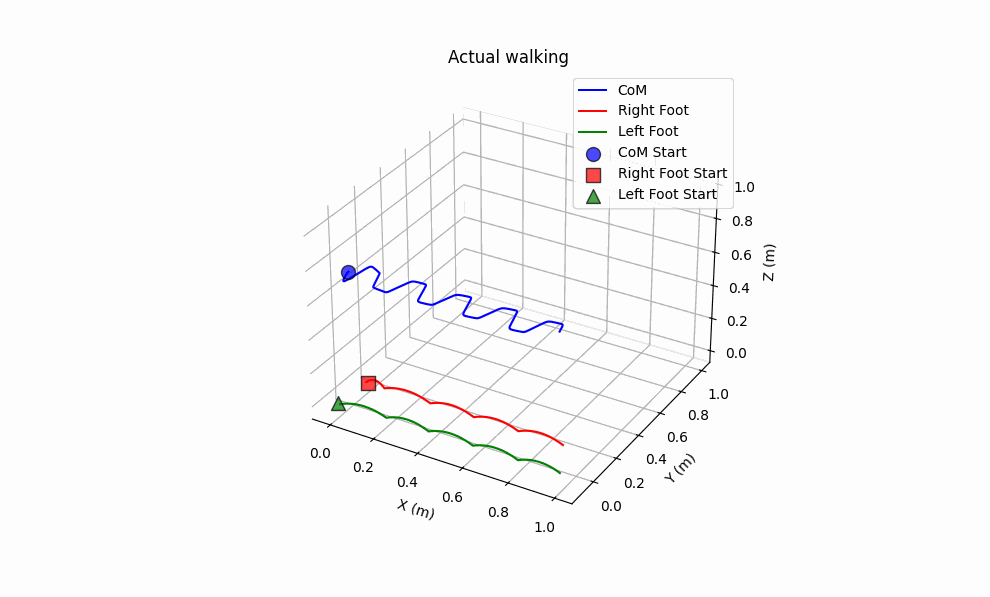
\includegraphics[width=0.8\textwidth]{figures/walking.PNG}
    \caption{Walking}
    \label{fig:walking}
\end{figure}


\end{document}



% OLD 

% \section{Simulation and Results}\label{sec:simulation}

% This section aims to visualize the results obtained with the proposed method. In the following, there is first defined the trajectory used for the task reference. Then, there are shown plots, tables and simulations.
% Before defining the trajectories implemented, let's denote with:
% \begin{itemize}
%     \item 0, when the foot is in contact with the surface
%     \item -, when the foot is off contact with the surface
% \end{itemize}
% The trajectories are defined with respect to contact point, not time.


% \subsection{Trajectory Generation}

% \subsubsection{Still Task}
% In this task the robot should not move at any instant of time and thus keeping the same initial position. 
% The contact sequence used is reported in Table ~\ref{tab:cs_still} where the first row concerns the right foot and the second row the left foot.
% \begin{table}[H]
% \label{tab:cs_still}
% \centering
% \begin{tabular}{|c|c|l|}
% \hline
% \textbf{Task} & \textbf{N} & \textbf{Contact Sequence} \\
% \hline
% Still & 3 & 
% \begin{tabular}[c]{@{}l@{}} 
% 0\,0\,0\ \\
% 0\,0\,0\ 
% \end{tabular} \\
% \hline
% \end{tabular}
% \caption{Contact sequence for still task}
% \end{table}

% The trajectory is simply defined as follows:
% \begin{algorithm}[H]
% \caption{Reference Trajectory Initialization and Update}
% \begin{algorithmic}[1]
% \State Initialize $X_{\text{ref}} \in \mathbb{R}^{28 \times (N+1)}$, $U_{\text{ref}} \in \mathbb{R}^{27 \times N}$
% \State Set initial CoM state, feet positions and orientations in $X_{\text{ref}}$
% \State $\text{time} \gets 0$, $\text{sig\_idx} \gets 0$

% \For{$t = 0$ to $N-1$}
%     \State Read contact states from $\sigma$
%     \State Set phase duration and contact force gains $\lambda$
%     \State Update $U_{\text{ref}}$ with phase duration and $\lambda$
%     \State $\text{sig\_idx} \gets \text{sig\_idx} + 2$
% \EndFor

% \For{$t = 1$ to $N$}
%     \State Set CoM velocity and feet step velocities as the initial state values (zeros)
%     \State Update CoM and feet positions based on velocity and duration
%     \State Update time and orientations in $X_{\text{ref}}$ as initial state
%     \State $\text{sig\_idx} \gets \text{sig\_idx} + 2$
% \EndFor

% \State \Return $X_{\text{ref}}, U_{\text{ref}}$
% \end{algorithmic}
% \end{algorithm}


% \subsubsection{Walking Task}
% For the walking task, the trajectory used relies on the following concepts:
% during the double-contact phases, in which both feet are on the ground, namely [0, 0], the COM does not move forward. Instead, it moves forward (along the X axis) only during single-support phases (a step), namely when right/left foot is lifting ([-, 0] or [0, -] respectively). Therefore if the preceding phase is a double support, the current phase COM keeps the same position as before, while if the preceding phase is of single support, the current phase COM has the previous position + some displacement; The Z (height) of each foot is always zero since at the beginning of each phase the feet are on the ground, while the X increases in an alternating manner depending on which foot was lifted in the previous phase. Also, the feet moves simulating a real walk, where the foot that is moving "surpasses" the one in contact, touching the ground beyond it, instead of positioning just next to the contact foot like before.
% Lastly, each foot is interpolated in the intra-phase height position by following a parabolic profile that starts and arrives at the corresponding positions given by the phases solutions, instead of using the fixed inputs (zero-hold).
% The contact sequence used is reported in Table ~\ref{tab:cs} where the first row concerns the right foot and the second row the left foot.
% \begin{table}[H]
% \label{tab:cs}
% \centering
% \begin{tabular}{|c|c|l|}
% \hline
% \textbf{Task} & \textbf{N} & \textbf{Contact Sequence} \\
% \hline
% Walk & 24 & 
% \begin{tabular}[c]{@{}l@{}} 
% 0\,0\,0\,-\,0\,0\,0\,-\,0\,0\,0\,-\,0\,0\,0\,-\,0\,0\,0\,-\,0\ \\
% 0\,-\,0\,0\,0\,-\,0\,0\,0\,-\,0\,0\,0\,-\,0\,0\,0\,-\,0\,0\,0 
% \end{tabular} \\
% \hline
% \end{tabular}
% \caption{Contact sequence for walking task}
% \end{table}
% The algorithm used for this task is shown below:


% \begin{algorithm}
% \caption{Reference Trajectory Initialization and Update}
% \begin{algorithmic}[1]
% \State Initialize $X_{\text{ref}} \in \mathbb{R}^{28 \times (N+1)}$, $U_{\text{ref}} \in \mathbb{R}^{27 \times N}$
% \State Set initial CoM state, feet positions and orientations in $X_{\text{ref}}$
% \State $\text{time} \gets 0$, $\text{sig\_idx} \gets 0$

% \For{$t = 0$ to $N-1$}
%     \State Read contact states from $\sigma$
%     \State Set phase duration and contact force gains $\lambda$
%     \State Update $U_{\text{ref}}$ with phase duration and $\lambda$
%     \State $\text{sig\_idx} \gets \text{sig\_idx} + 2$
% \EndFor

% \For{$t = 1$ to $N$}
%     \State Read current and previous contact states
%     \State Set CoM velocity $(v_x, v_y)$ and feet step velocities
%     \State Update CoM and feet positions based on velocity and duration
%     \State Update time and orientations in $X_{\text{ref}}$
%     \State $\text{sig\_idx} \gets \text{sig\_idx} + 2$
% \EndFor

% \State \Return $X_{\text{ref}}, U_{\text{ref}}$
% \end{algorithmic}
% \end{algorithm}


% \subsection{Solutions}
% Solutions of those problems and tasks are tuples (X, U) where X is the state vector with dimension N , and U is the input vector with dimension N-1.
% \\The solution is computed with ipopt solver from Casadi optimizer. Both the reference and solution are contact-dependent, meaning that X and U contain values for each contact phase, thus to find the time dependent solution we used the dynamics. 

% \subsection{Still Task: results}
% In this case the state vector has dimension 3, and the input vector has dimension 2.
% \subsubsection{CoM Plots}
% The following plots report the CoM trajectory in time. 
% The alternation between light and dark grey on the background suggests the switch between phases.
% As plots suggest there's no significant motion in any direction.
% \begin{figure}[H]
%     \centering
%     \begin{subfigure}[b]{0.45\textwidth}
%         \centering
%         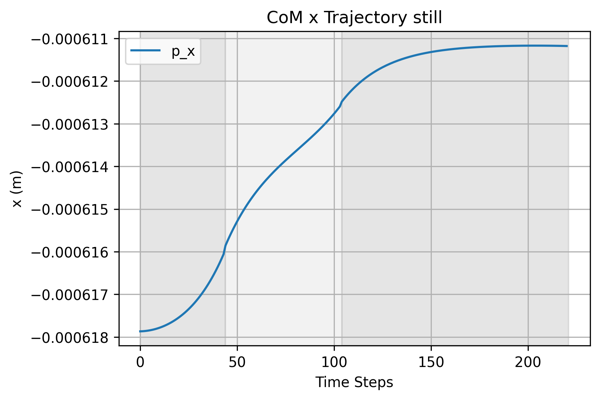
\includegraphics[width=\textwidth]{figures/CoM x Trajectory still.png}
%         \caption{Com X Trajectory 1}
%         \label{fig:sub1_still}
%     \end{subfigure}
%     \hfill
%     \begin{subfigure}[b]{0.45\textwidth}
%         \centering
%         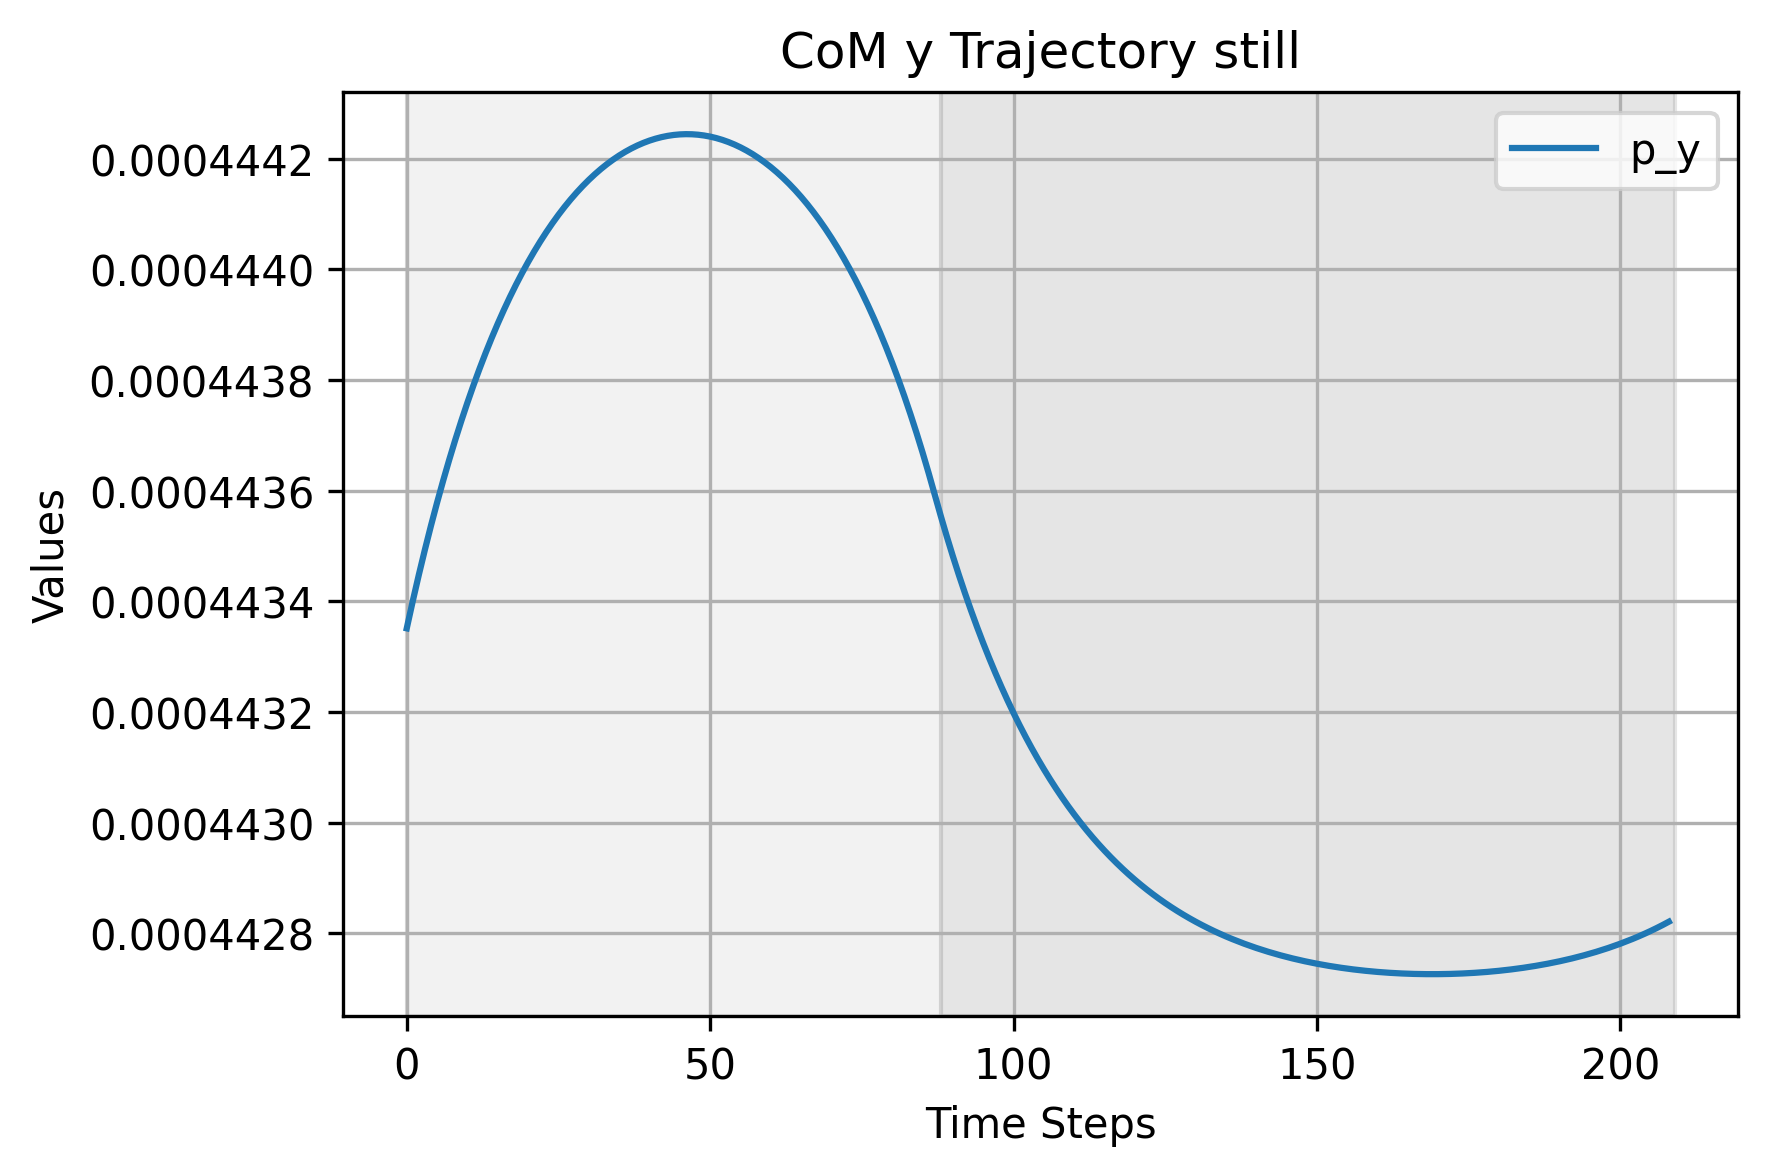
\includegraphics[width=\textwidth]{figures/CoM y Trajectory still.png}
%         \caption{Com Y Trajectory 1}
%         \label{fig:sub2_still}
%     \end{subfigure}
%     \hfill
%     \begin{subfigure}[b]{0.45\textwidth}
%         \centering
%         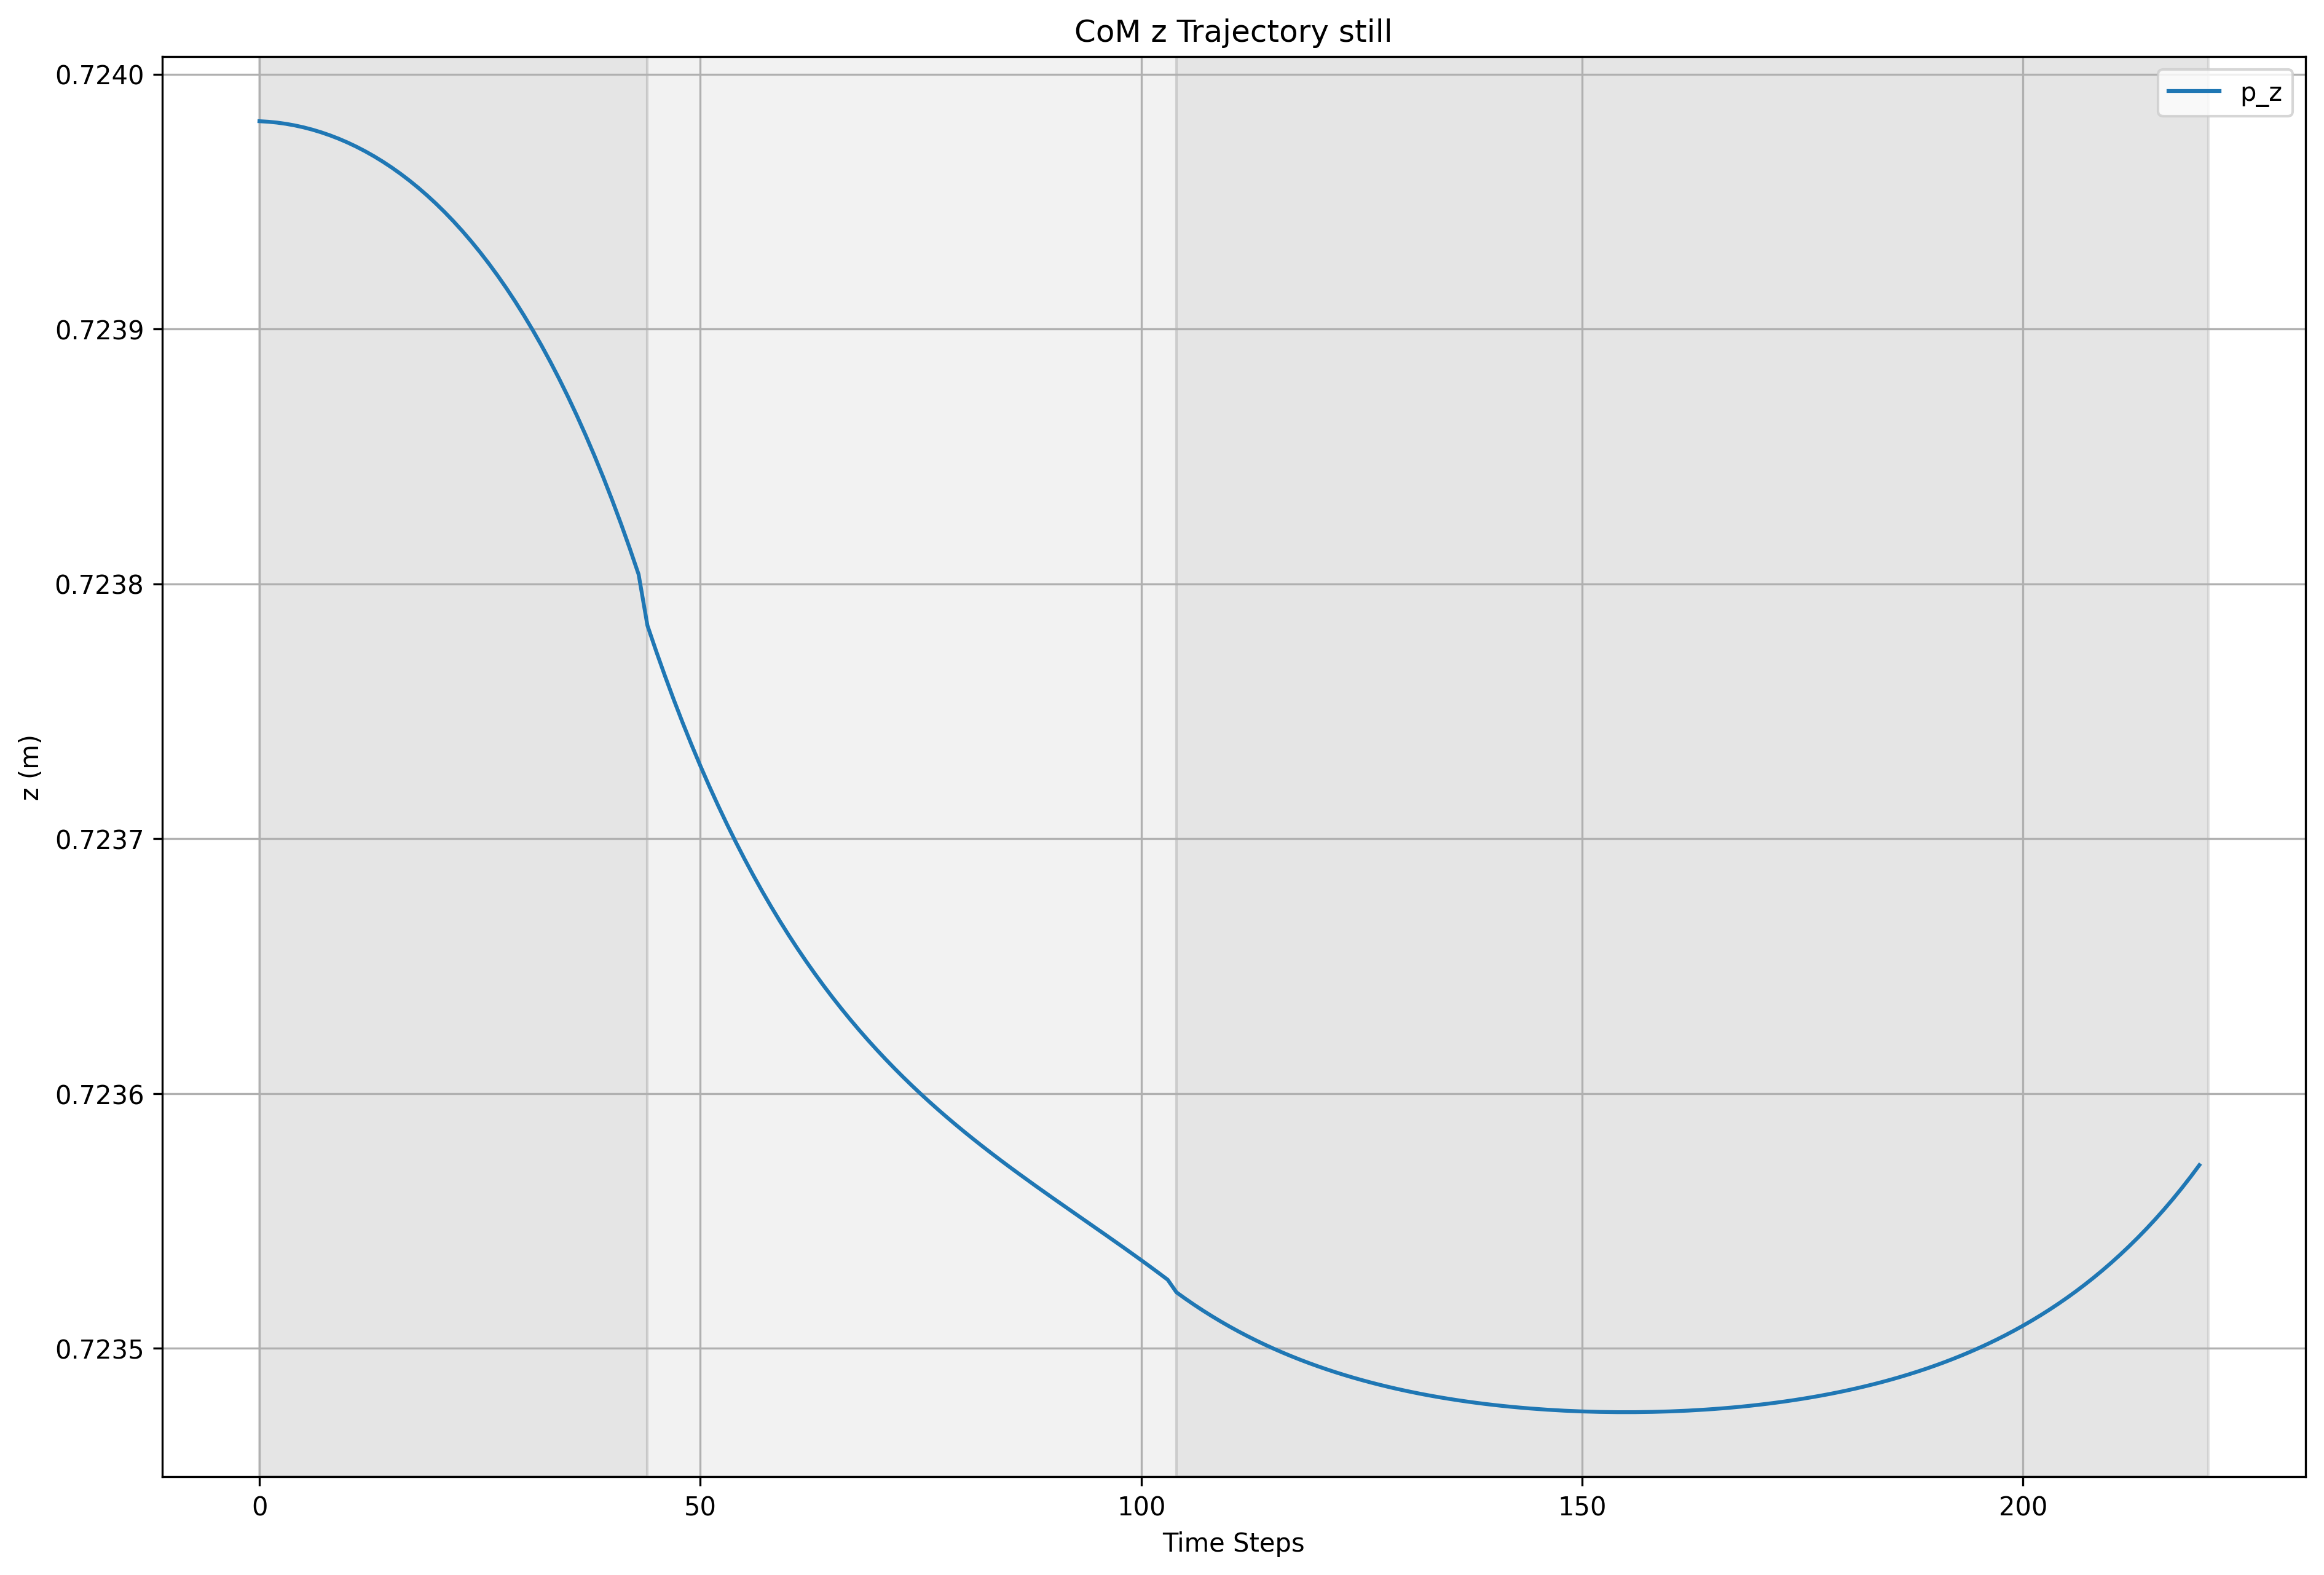
\includegraphics[width=\textwidth]{figures/CoM z Trajectory still.png}
%         \caption{Com Z Trajectory 1}
%         \label{fig:sub3_still}
%     \end{subfigure}
%     \caption{Com Trajectory}
%     \label{fig:threeimages_still}
% \end{figure}

% \begin{figure}[htbp]
%     \centering
%     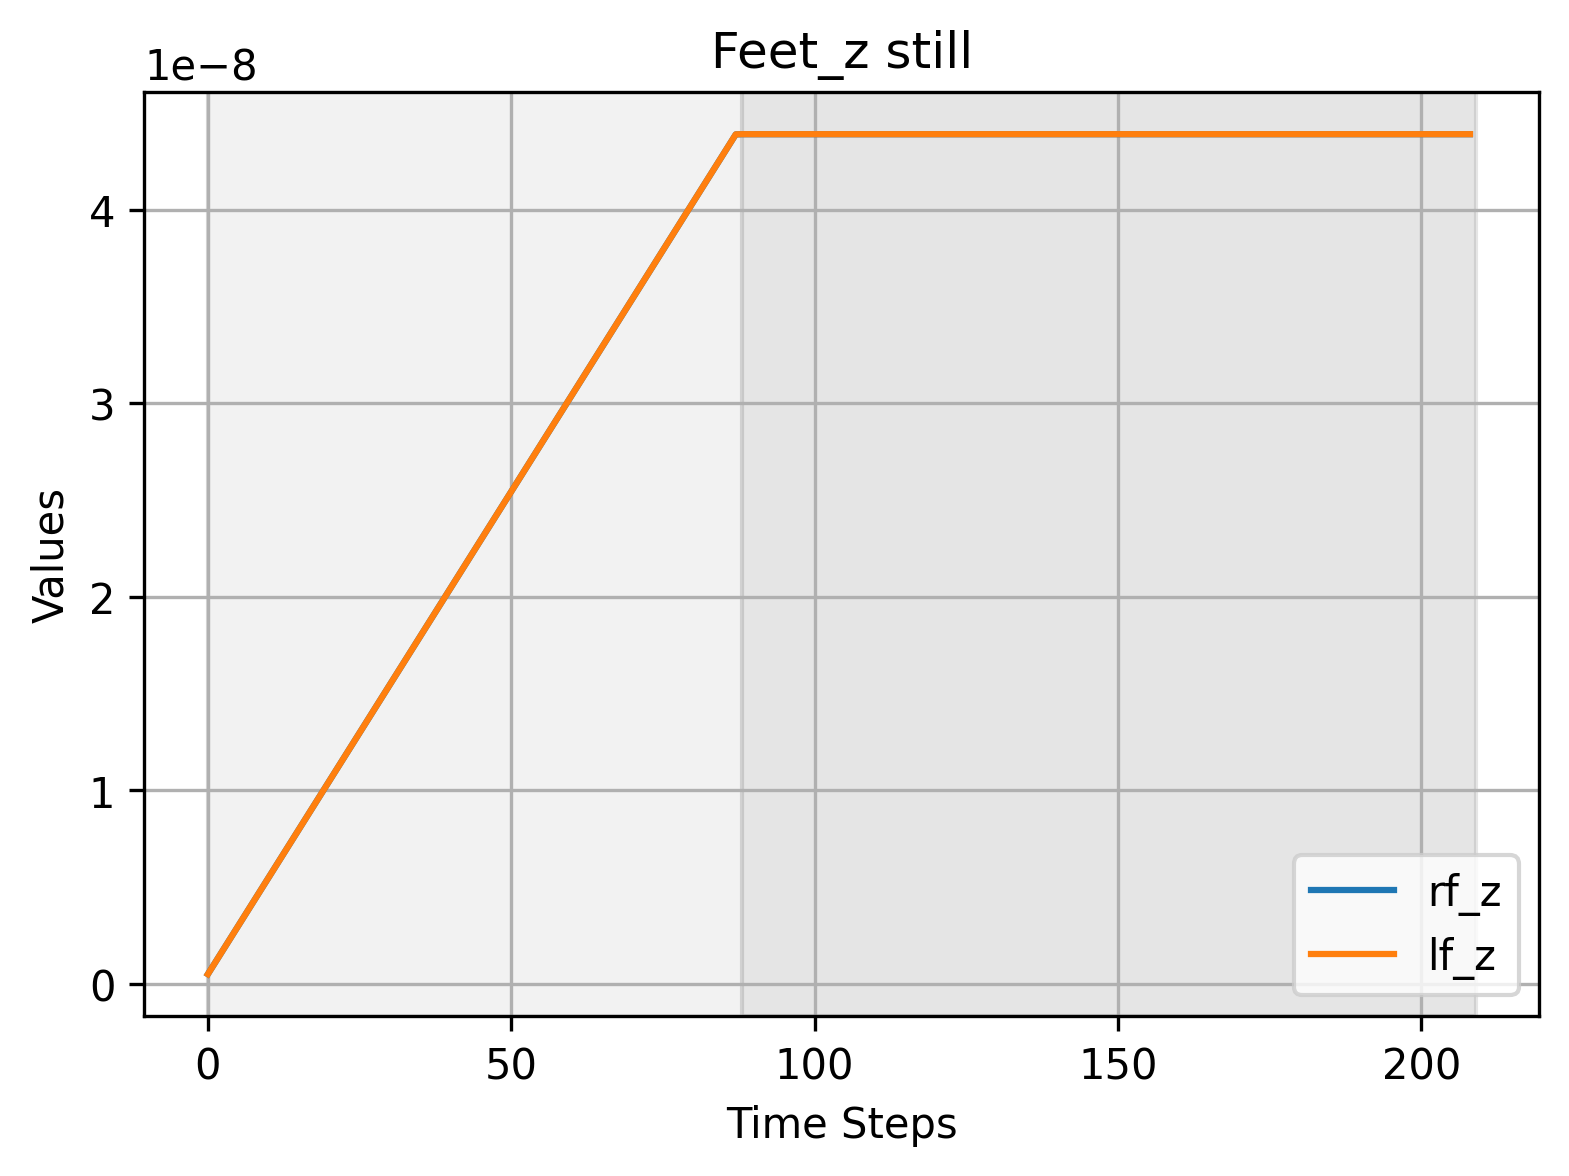
\includegraphics[width=0.6\textwidth]{figures/Feet_z still.png}
%     \caption{Feet along Z}
%     \label{fig:feet_still}
% \end{figure}


% \subsubsection{State and Input Contact Values}
% In the following plots, the main components of the state and input vectors solutions are compared with the reference at each contact step.
% \begin{figure}[htbp]
%     \centering
%     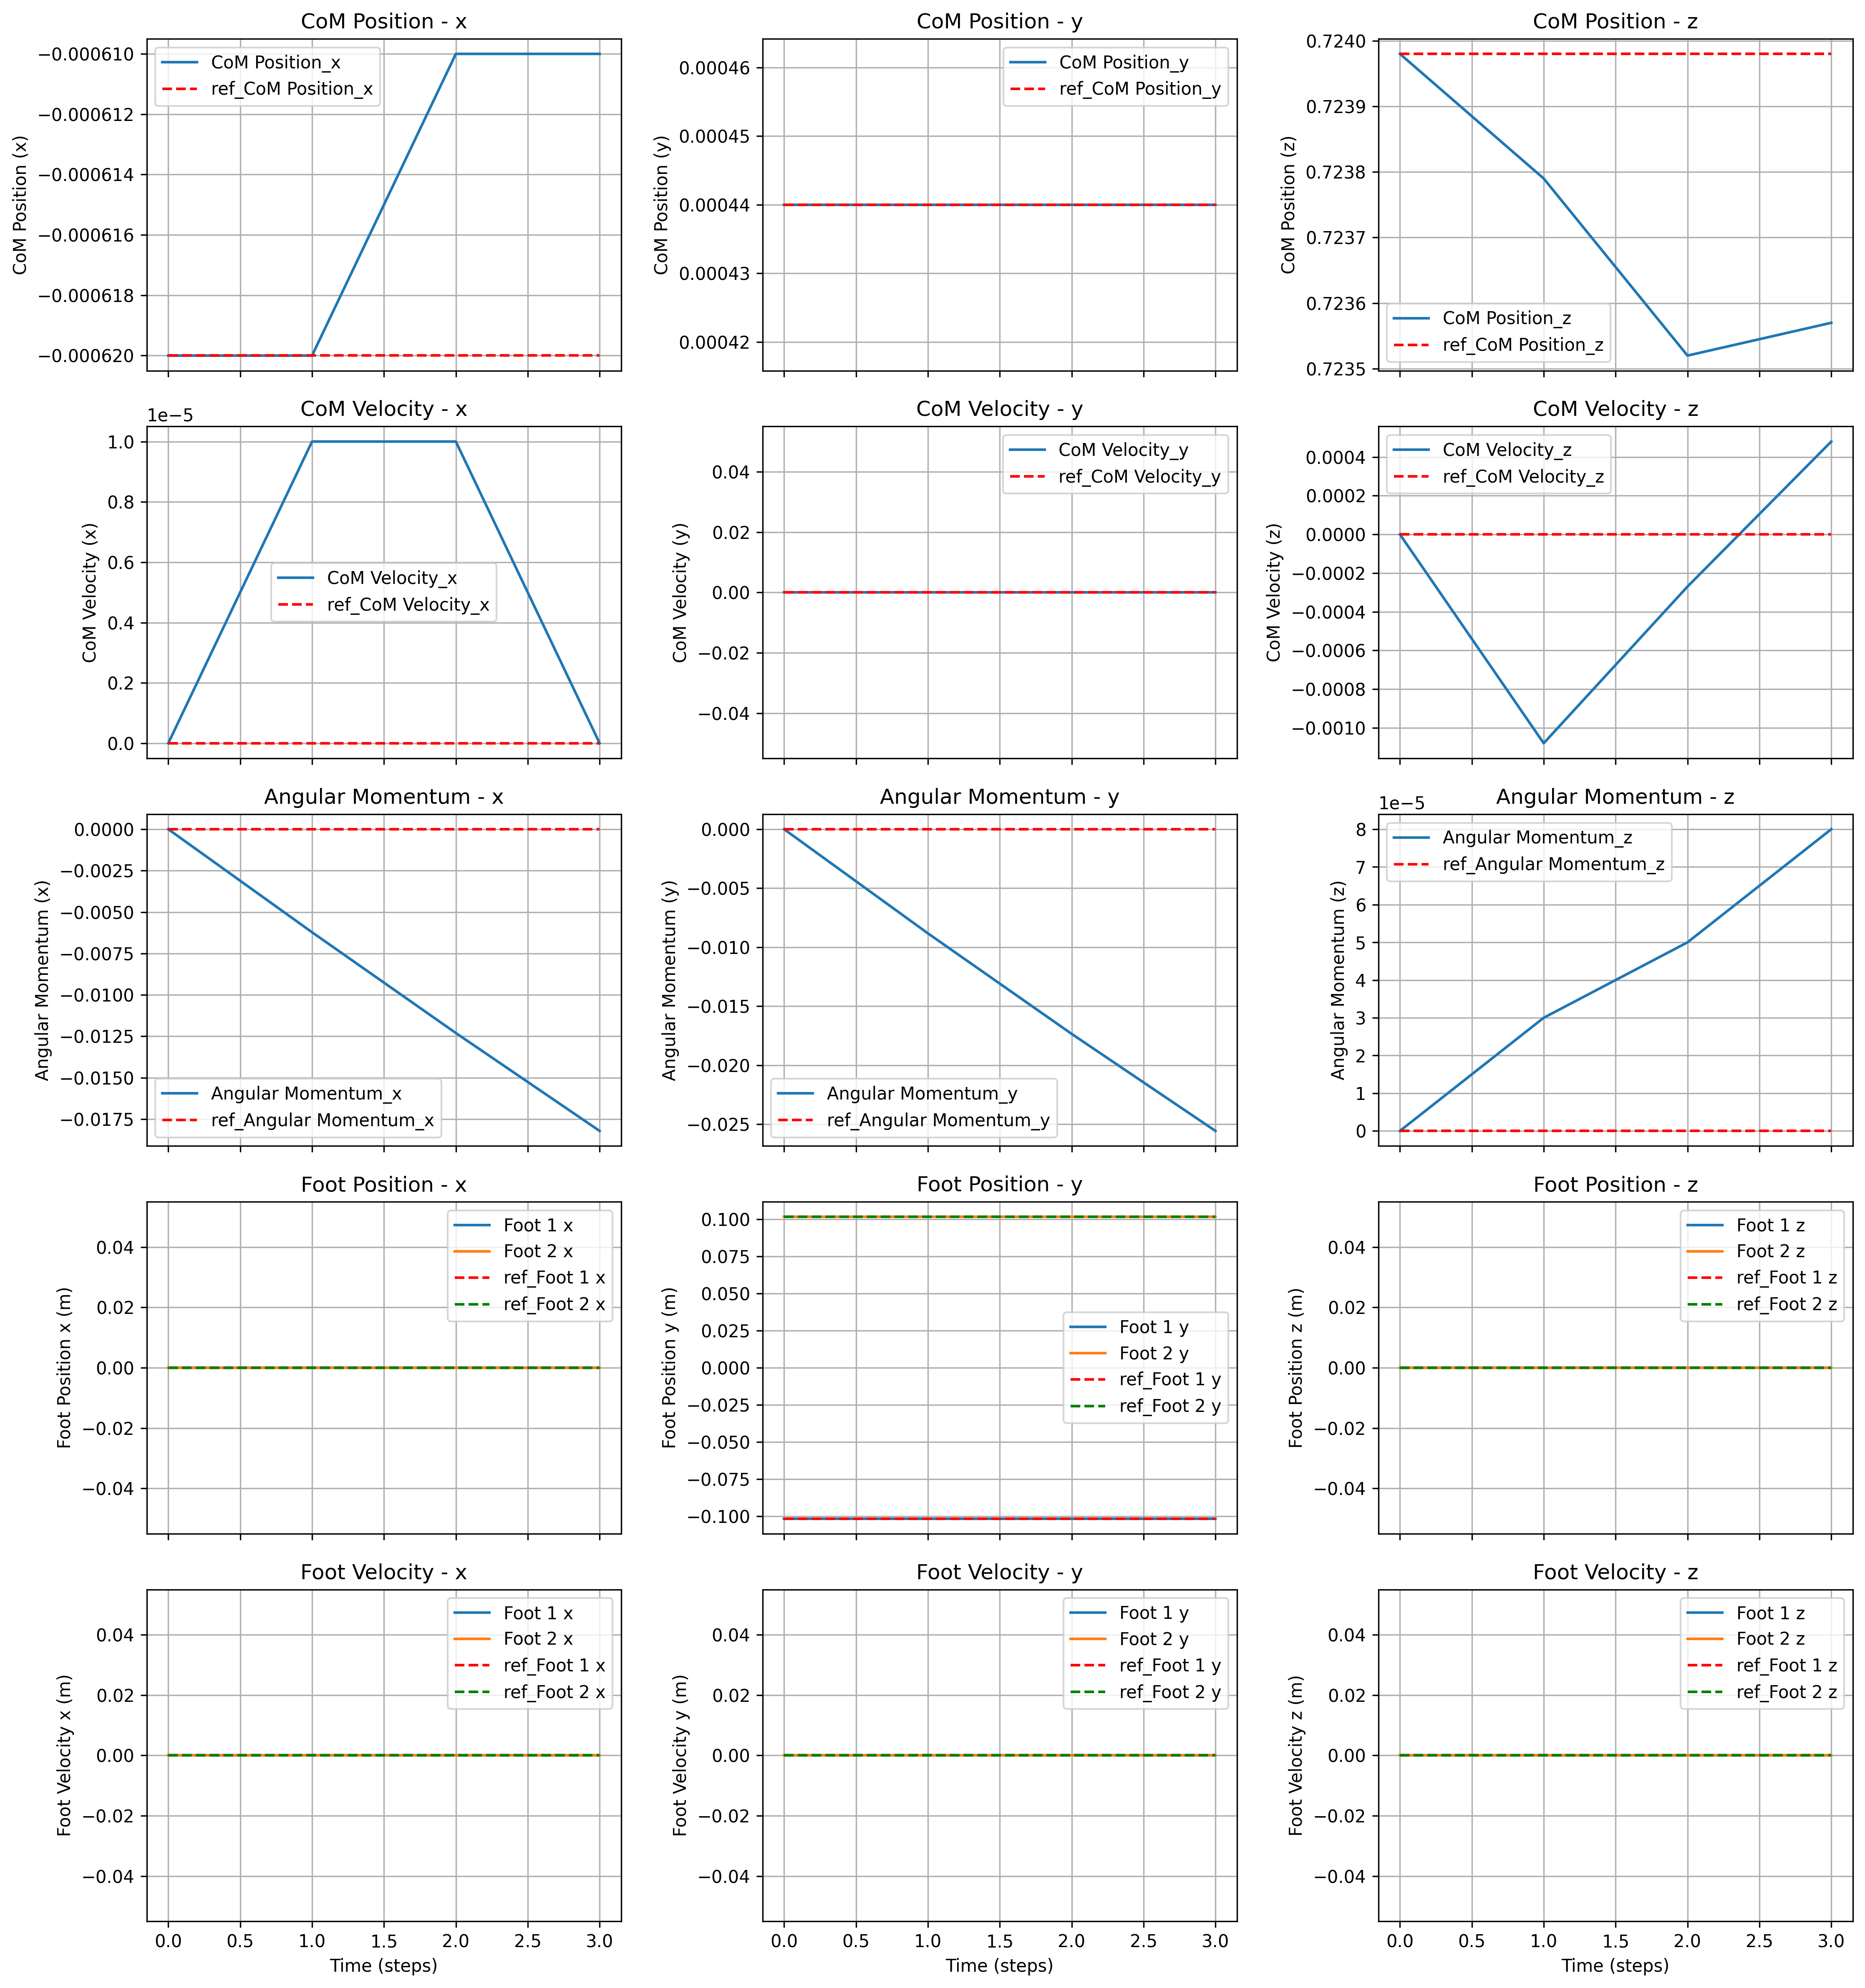
\includegraphics[width=0.6\textwidth]{figures/contact_x_still.png}
%     \caption{Trajectory vs Reference: state vector}
%     \label{fig:contact_x_still}
% \end{figure}

% \subsubsection{Contact Forces}
% Another important dynamic aspect regards forces. 
% In the input vector, the contact wrench that describes all the mechanical influence that a contact point (like a foot or hand) exerts on the robot or vice versa.
% To balance dynamic laws, along the Z-axis the environment should exert a reaction force equal to the gravity factor multiplied by the mass of the robot. In the table ~\ref{tab:contact_forces_still}  below there are listed the contact forces exerting from the environment to both feet. As the table shows, when both feet are on the ground the gravity force is equally distributed on left and right foot.
% \begin{table}[H]
% \label{tab:contact_forces_still}
% \centering
% \begin{tabular}{ccc}
% \toprule
% Right Foot Z & Left Foot Z & $\Sigma_L^k$ \\
% \midrule
% 49.0644 & 49.0531 & [0., 0.] \\
% 48.8973 & 49.65 & [0., 0.] \\
% \bottomrule
% \end{tabular}
% \caption{Z-axis gravity force and $\Sigma_L^k$ values}
% \end{table}

% Components of contact wrench, rotational and translational forces, are graphically expressed in the following plots:
% \begin{figure}[htbp]
%     \centering
%     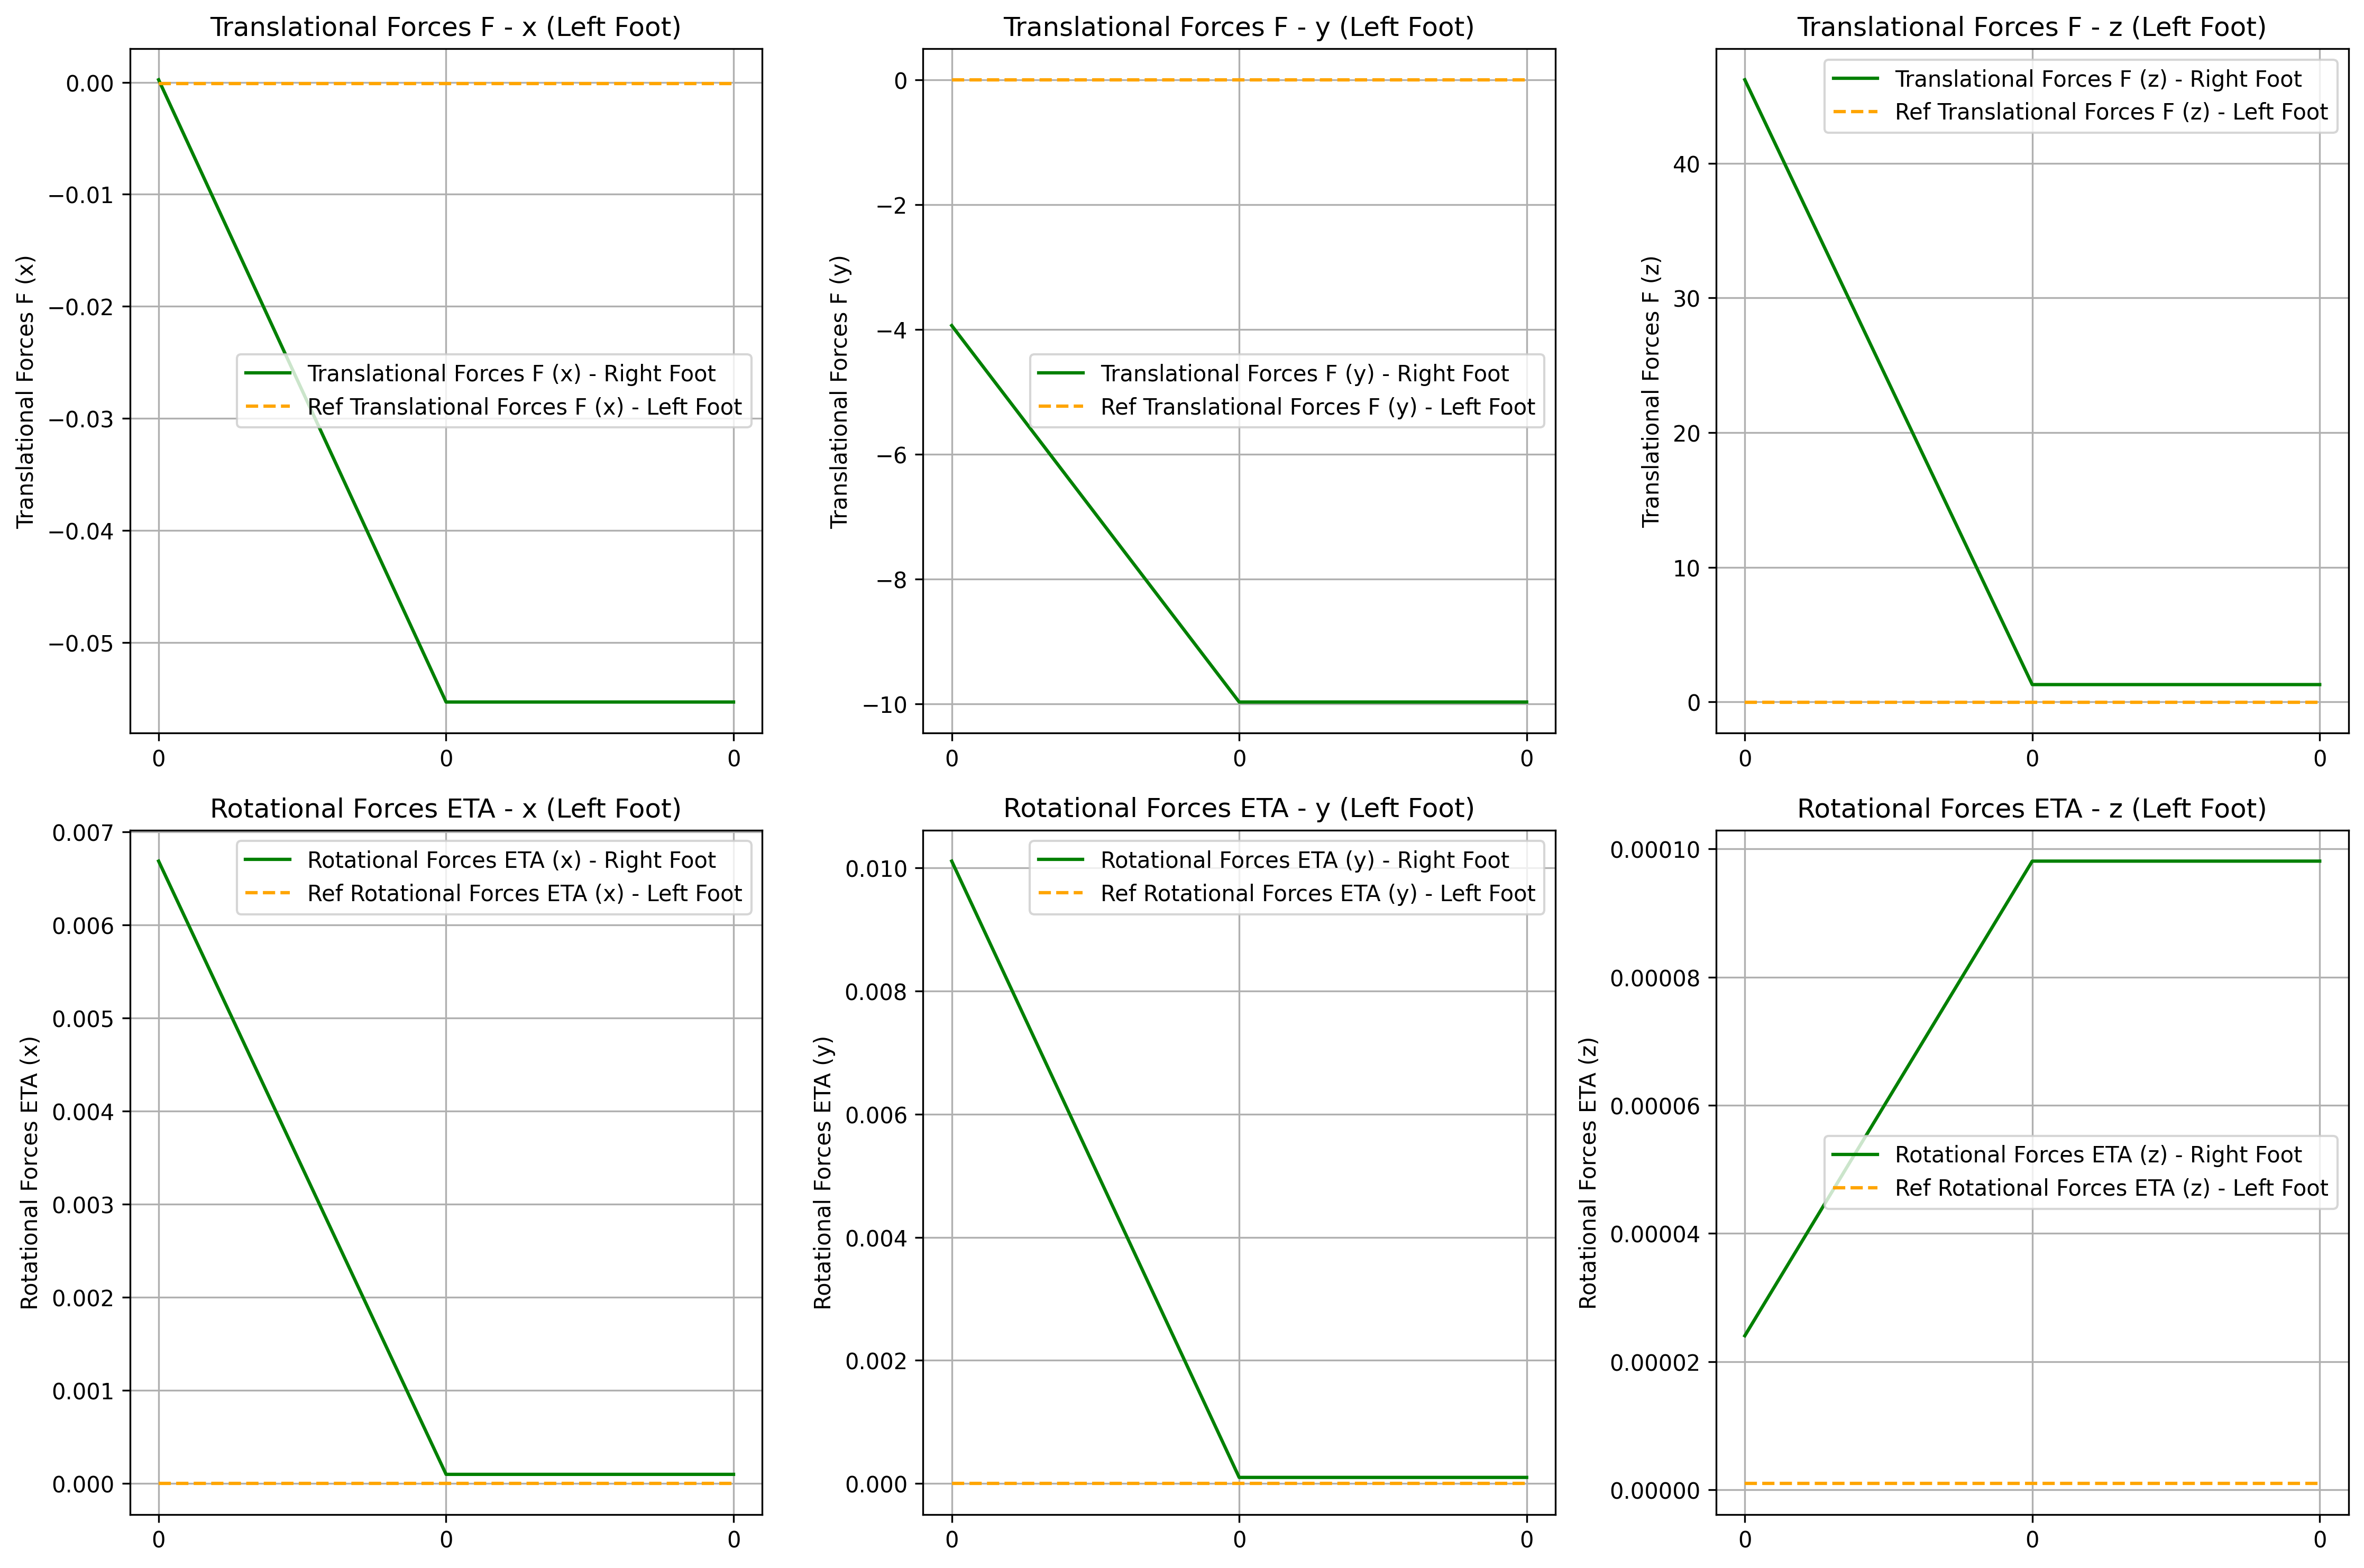
\includegraphics[width=0.8\textwidth]{figures/contact_forces_still.png}
%     \caption{Trajectory vs Reference: Forces}
%     \label{fig:contact_forces_still}
% \end{figure}

% \newpage
% \subsubsection{Robot representation}
% In this section it is possible to visualize first the path followed by the CoM, right and left foot in time:
% \begin{figure}[htbp]
%     \centering
%     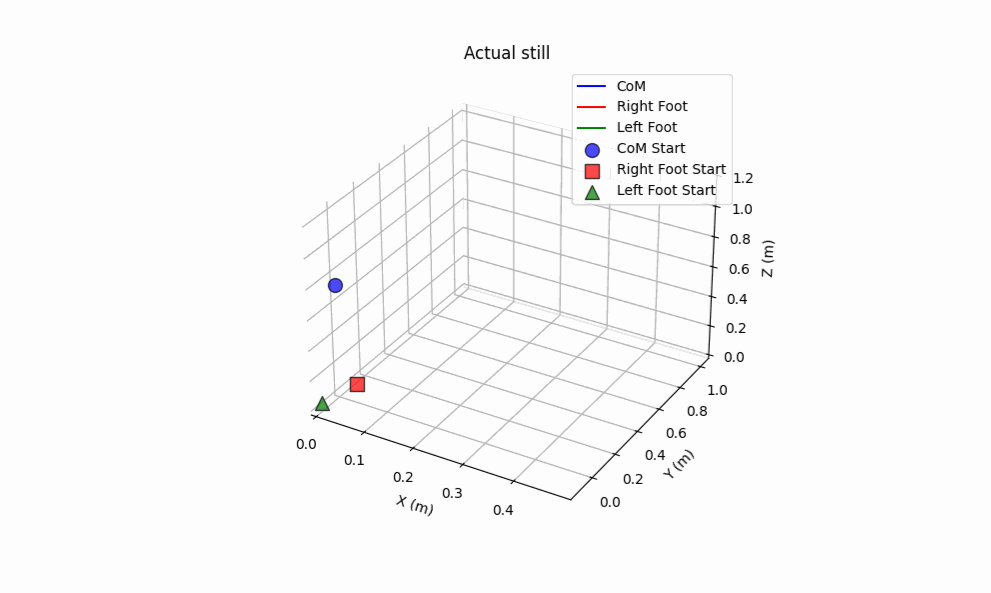
\includegraphics[width=0.8\textwidth]{figures/still.PNG}
%     \caption{Still}
%     \label{fig:still}
% \end{figure}


% \subsection{Walking Task: results}
% In this case the state vector has dimension 24 and the input vector has dimension 23.


% \subsubsection{CoM Plots}
% The following plots report the CoM trajectory in time. 
% The alternation between light and dark grey on the background suggests the switch between phases.
% As Fig. ~\ref{fig:sub1} shows, the CoM exhibits linear motion in the x-direction.
% Along the y-axis ~\ref{fig:sub2} the CoM goes towards the foot staying on the ground when lifting the other. Let's consider the first two contacts: in the first one, the robot is in double support (both feet are on the ground), while the second one expects the left foot to raise. Infact, the CoM at the end of the first phase has moved towards the right foot. This mechanism is repeated through all the alternances between double support and single support.
% In the z-direction ~\ref{fig:sub3}, the CoM goes up and down in a small range of motion.
% \begin{figure}[H]
%     \centering
%     \begin{subfigure}[b]{0.45\textwidth}
%         \centering
%         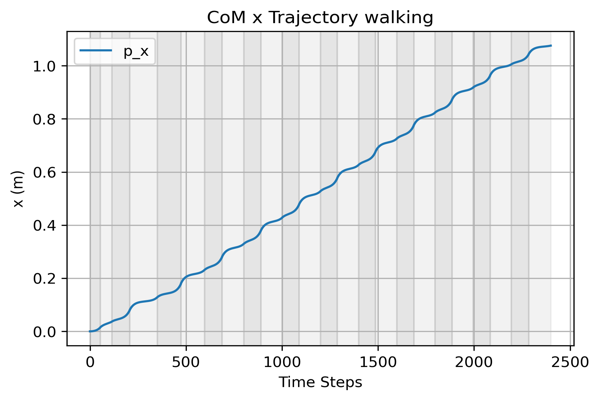
\includegraphics[width=\textwidth]{figures/CoM x Trajectory walking.png}
%         \caption{Com X Trajectory 1}
%         \label{fig:sub1_walking}
%     \end{subfigure}
%     \hfill
%     \begin{subfigure}[b]{0.45\textwidth}
%         \centering
%         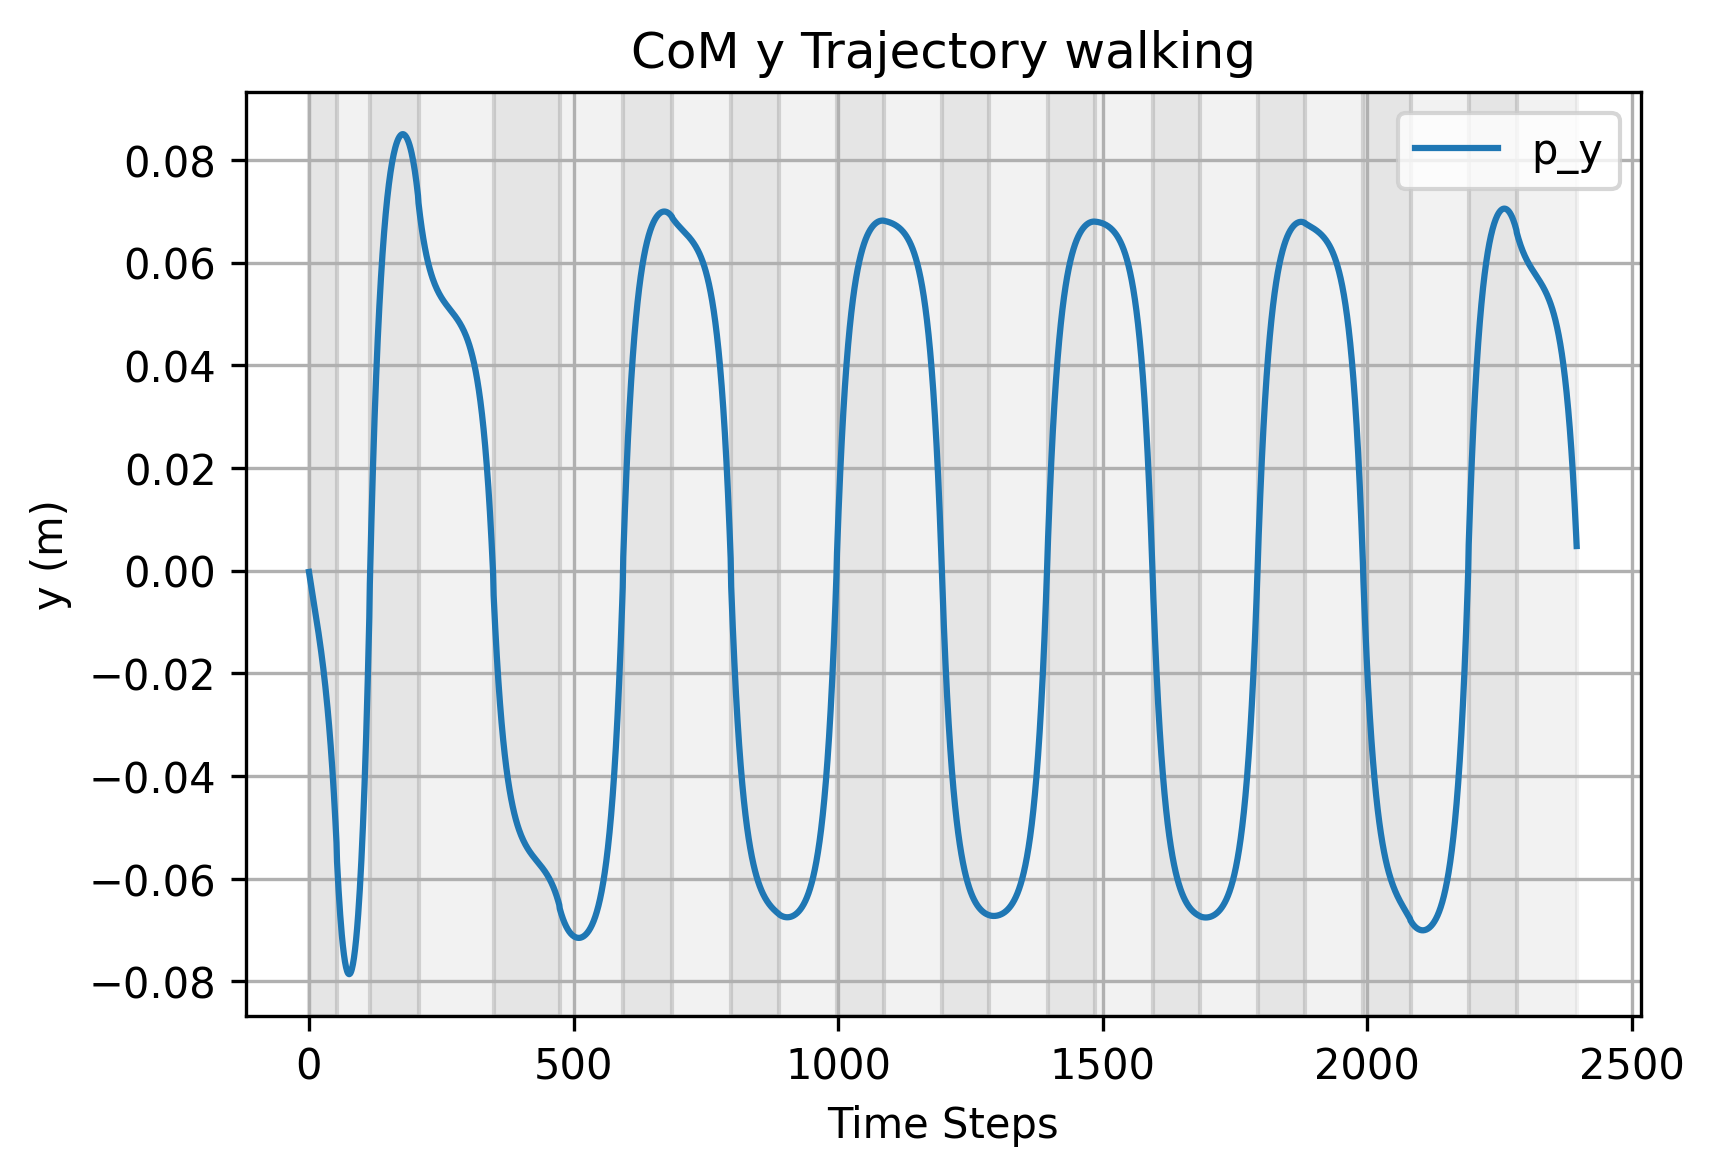
\includegraphics[width=\textwidth]{figures/CoM y Trajectory walking.png}
%         \caption{Com Y Trajectory 1}
%         \label{fig:sub2_walking}
%     \end{subfigure}
%     \hfill
%     \begin{subfigure}[b]{0.45\textwidth}
%         \centering
%         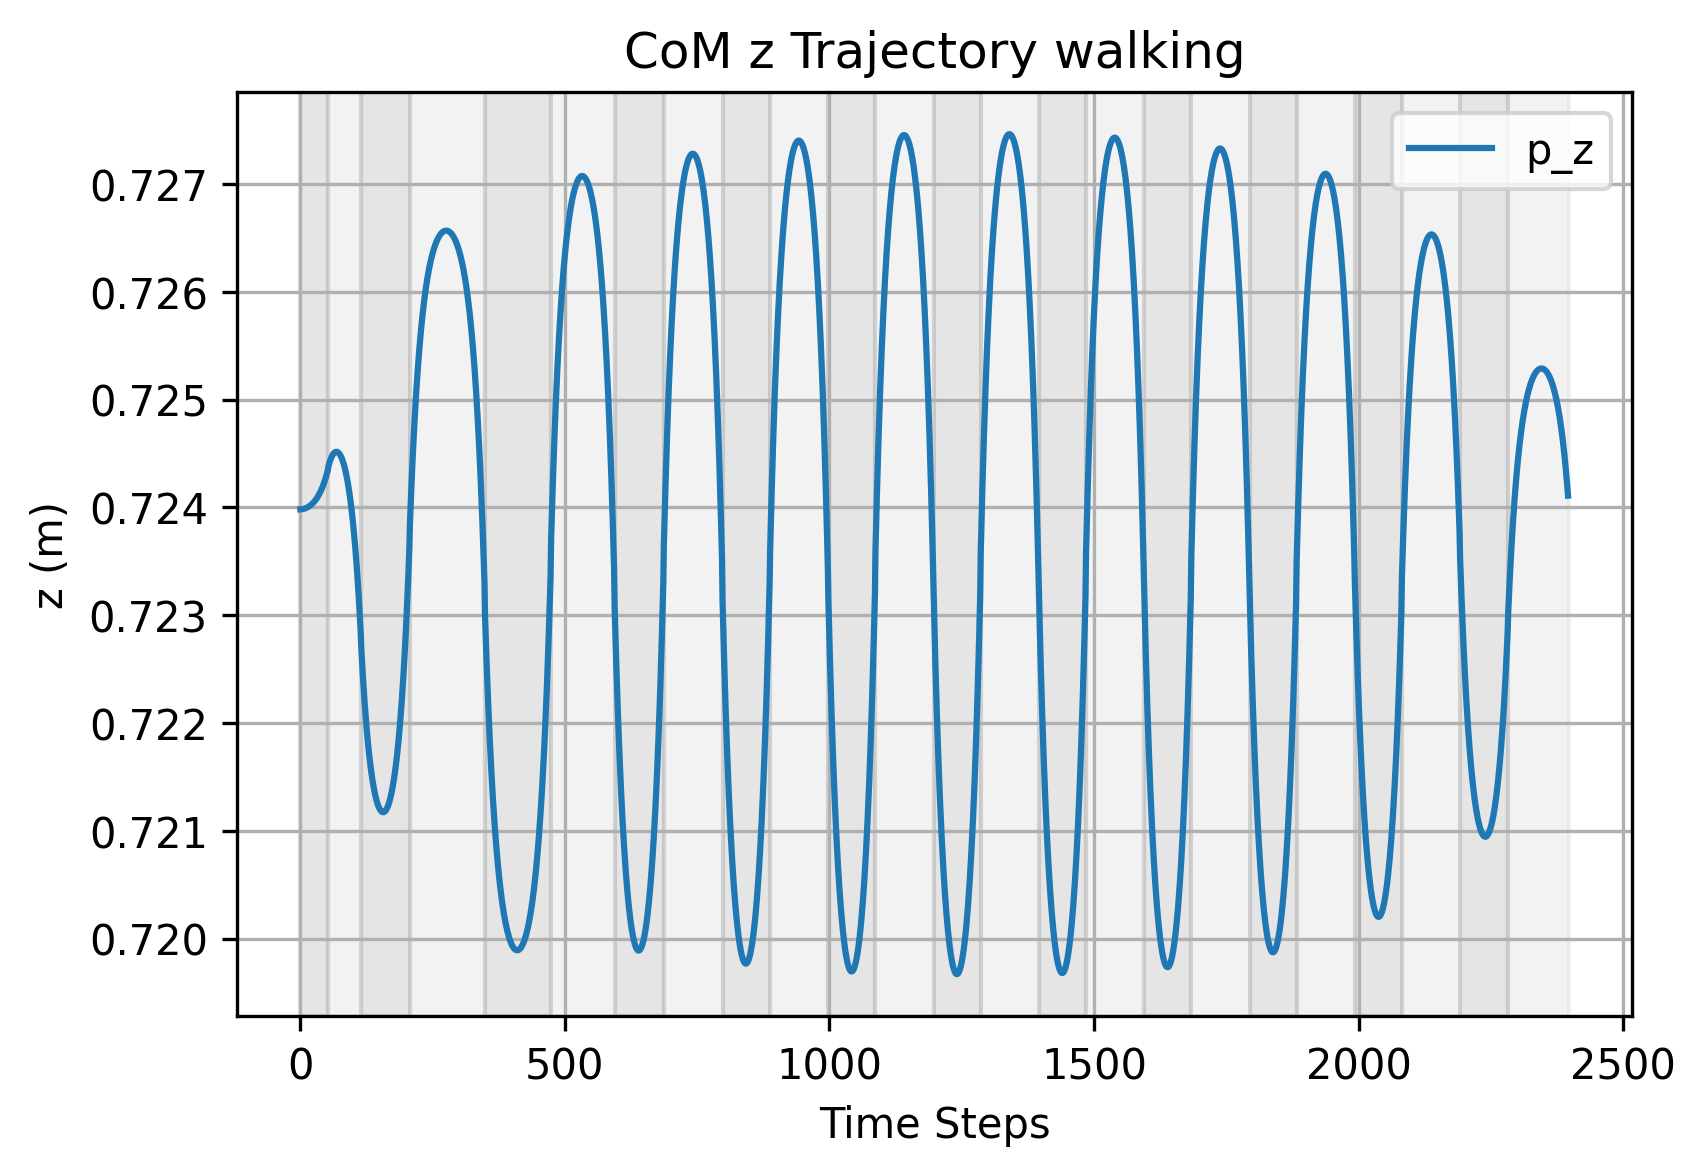
\includegraphics[width=\textwidth]{figures/CoM z Trajectory walking.png}
%         \caption{Com Z Trajectory 1}
%         \label{fig:sub3_walking}
%     \end{subfigure}
%     \caption{Com Trajectory}
%     \label{fig:threeimages_walking}
% \end{figure}
% Furthermore, the image below represent the foot position along the Z-axis in time. As one can see, they follow a parabolic profile.  
% \begin{figure}[htbp]
%     \centering
%     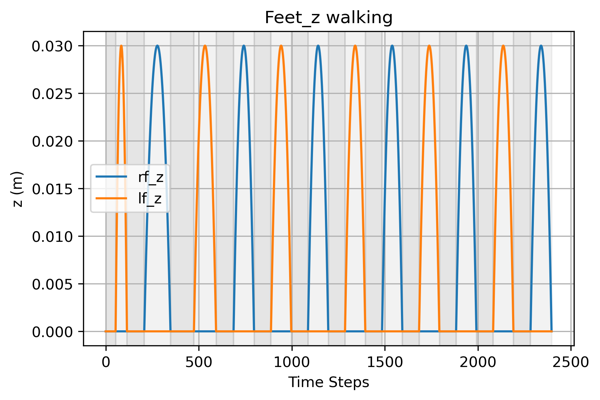
\includegraphics[width=0.6\textwidth]{figures/Feet_z walking.png}
%     \caption{Feet along Z}
%     \label{fig:feet_walking}
% \end{figure}


% \subsubsection{State and Input Contact Values}
% In the following plots, the main components of the state and input vectors solutions are compared with the reference at each contact step.
% \begin{figure}[htbp]
%     \centering
%     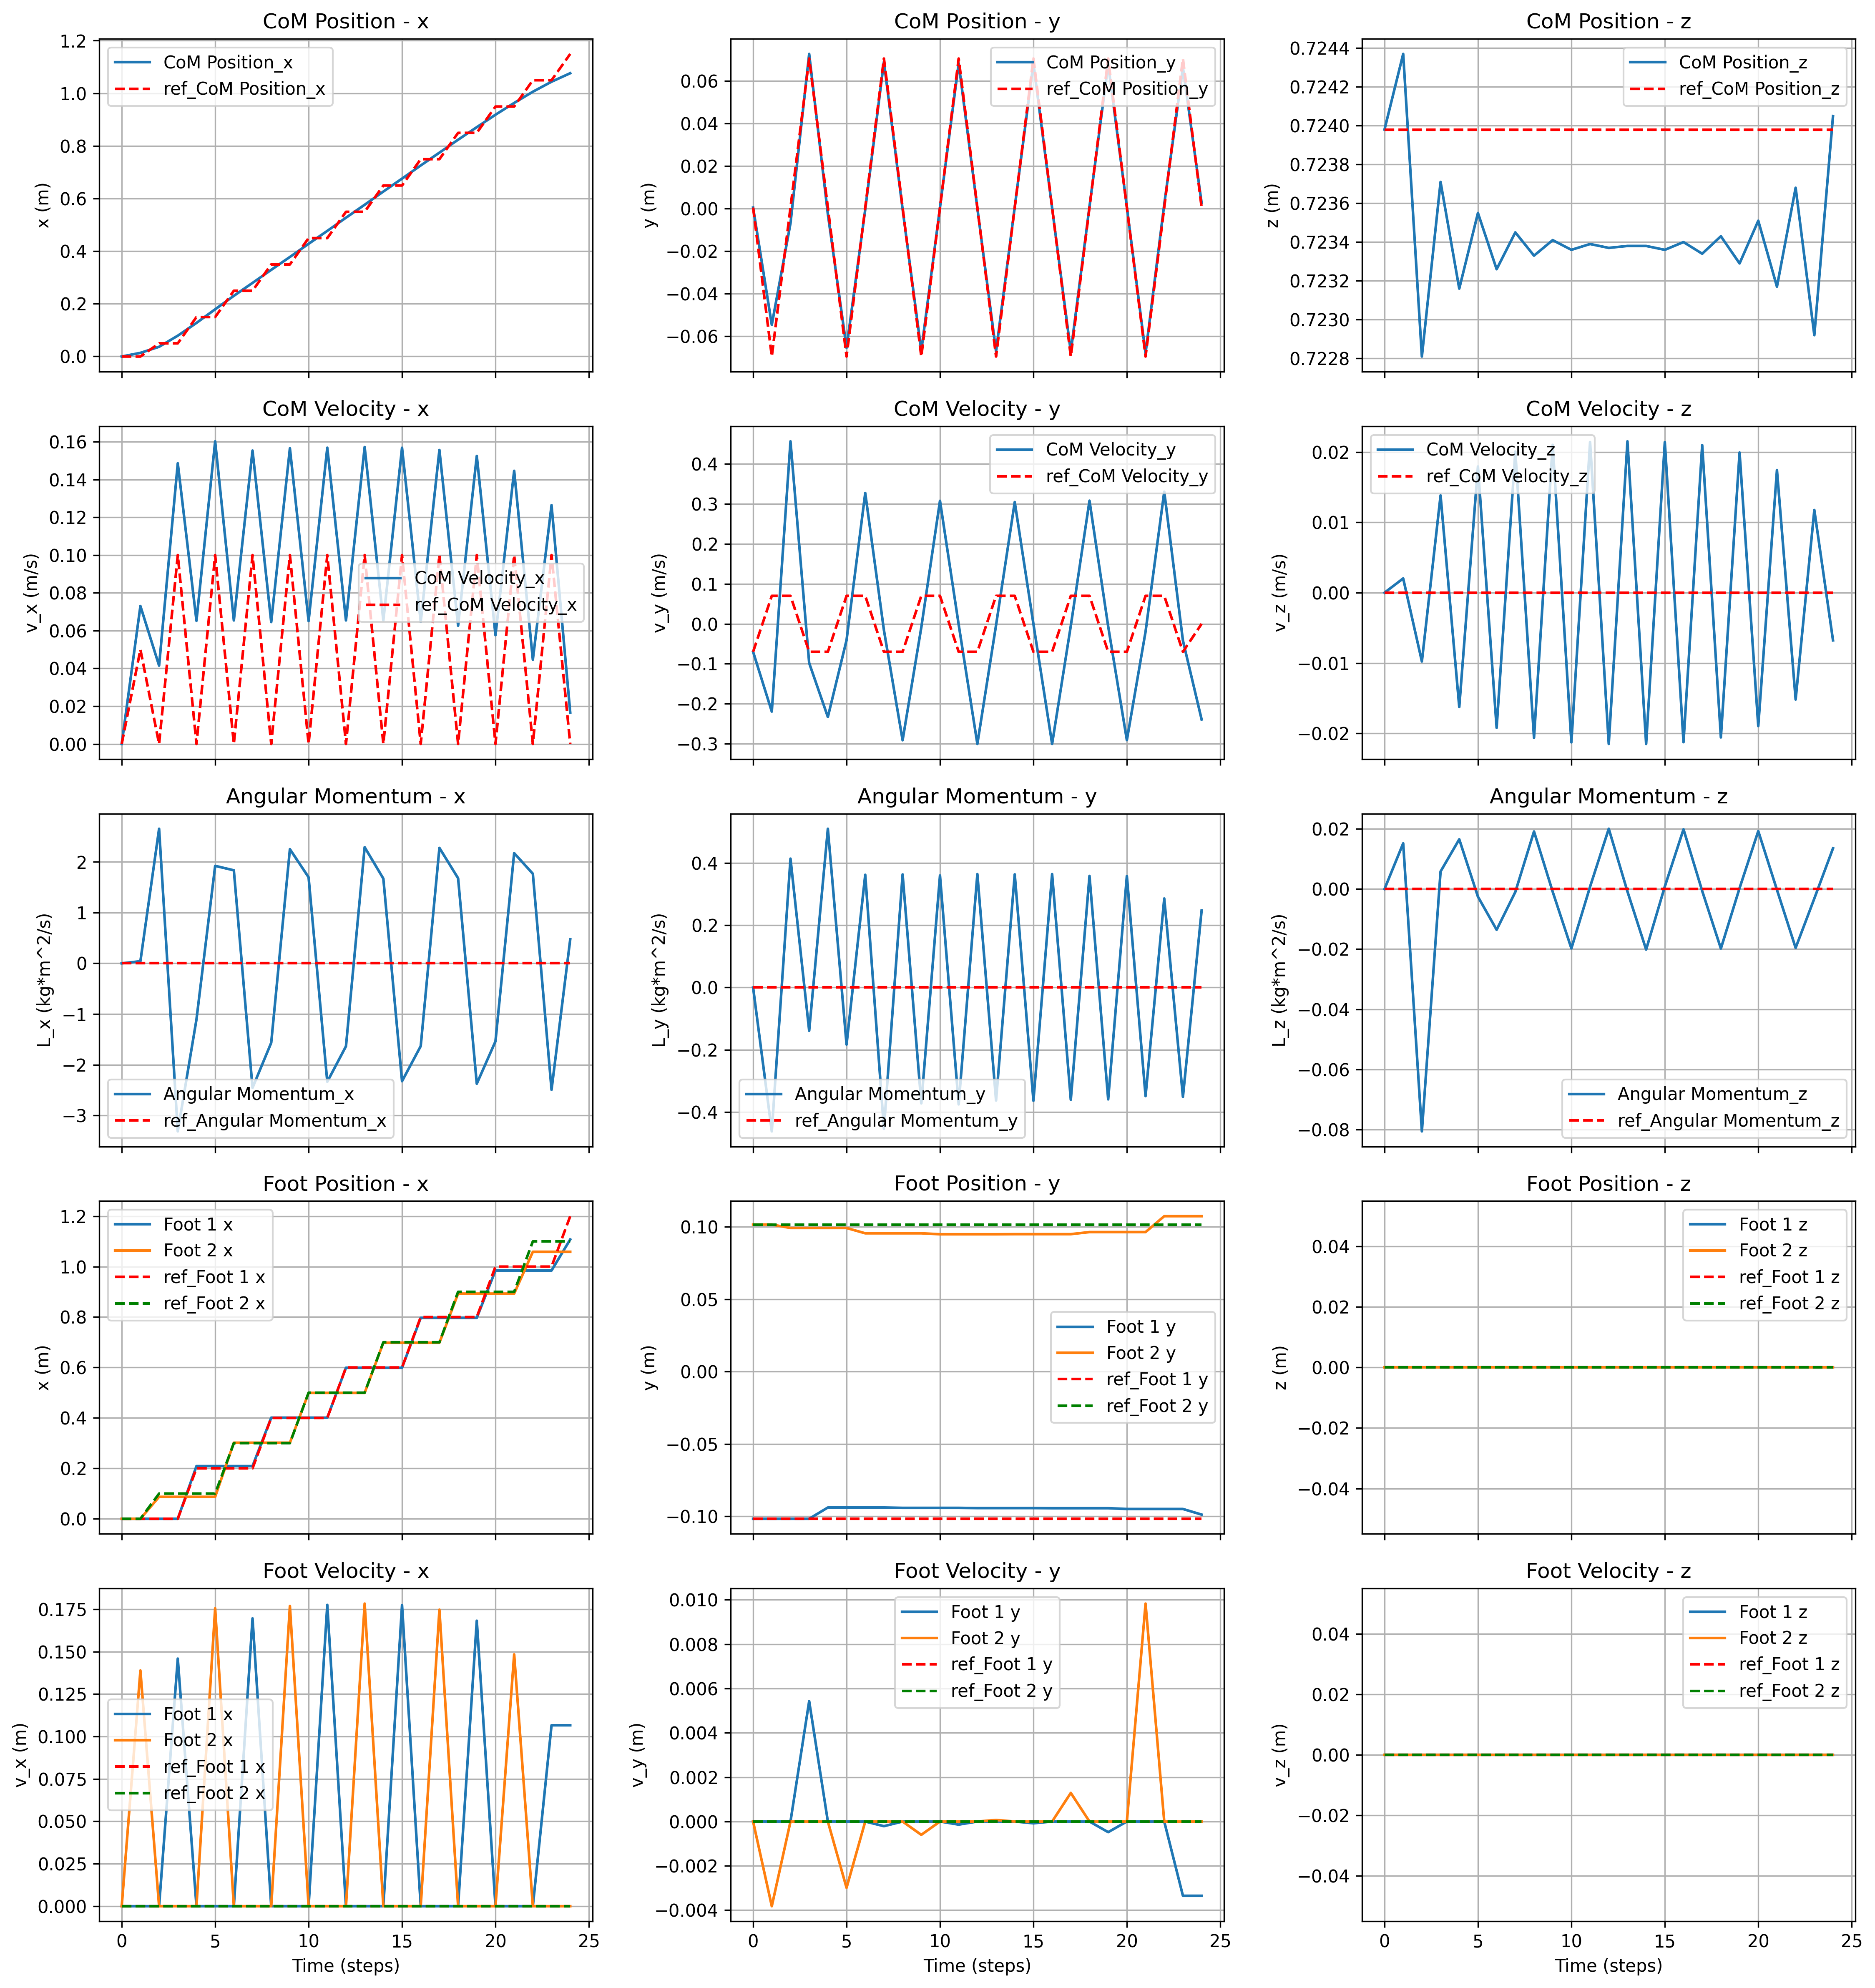
\includegraphics[width=0.6\textwidth]{figures/contact_x_walking.png}
%     \caption{Trajectory vs Reference: state vector}
%     \label{fig:contact_x_walking}
% \end{figure}

% \subsubsection{Contact Forces}
% Another important dynamic aspect regards forces. 
% In the input vector, the contact wrench that describes all the mechanical influence that a contact point (like a foot or hand) exerts on the robot or vice versa.
% To balance dynamic laws, along the Z-axis the environment should exert a reaction force equal to the gravity factor multiplied by the mass of the robot. In the table ~\ref{tab:contact_forces_walking}  below there are listed the contact forces exerting from the environment to both feet. As the table shows, when both feet are on the ground the gravity force is equally distributed on left and right foot, while when one foot lifts the gravity force acts only on the foot staying on the ground.
% \begin{table}[H]
% \label{tab:contact_forces_walking}
% \centering
% \begin{tabular}{ccc}
% \toprule
% Right Foot Z & Left Foot Z & $\Sigma_L^k$ \\
% \midrule
% 49.0644 & 49.0531 & [0., 0.] \\
% 97.9551 & 0 & [0., -] \\
% 48.8973 & 49.65 & [0., 0.] \\
% 0 & 97.4904 & [-, 0.] \\
% 49.6528 & 49.1563 & [0., 0.] \\
% 97.3081 & 0 & [0., -] \\
% 49.2399 & 49.7241 & [0., 0.] \\
% 0 & 97.2091 & [-, 0.] \\
% 49.7388 & 49.293 & [0., 0.] \\
% 97.1669 & 0 & [0., -] \\
% 49.3007 & 49.7613 & [0., 0.] \\
% 0 & 97.1486 & [-, 0.] \\
% 49.762 & 49.31 & [0., 0.] \\
% 97.1443 & 0 & [0., -] \\
% 49.3062 & 49.7655 & [0., 0.] \\
% 0 & 97.1495 & [-, 0.] \\
% 49.7557 & 49.3045 & [0., 0.] \\
% 97.1685 & 0 & [0., -] \\
% 49.2815 & 49.7467 & [0., 0.] \\
% 0 & 97.216 & [-, 0.] \\
% 49.7003 & 49.254 & [0., 0.] \\
% 97.3264 & 0 & [0., -] \\
% 49.1286 & 49.6485 & [0., 0.] \\
% 0 & 97.5828 & [-, 0.] \\
% \bottomrule
% \end{tabular}
% \caption{Z-axis gravity force and $\Sigma_L^k$ values}
% \end{table}

% Components of contact wrench, rotational and translational forces, are graphically expressed in the following plots:
% \begin{figure}[htbp]
%     \centering
%     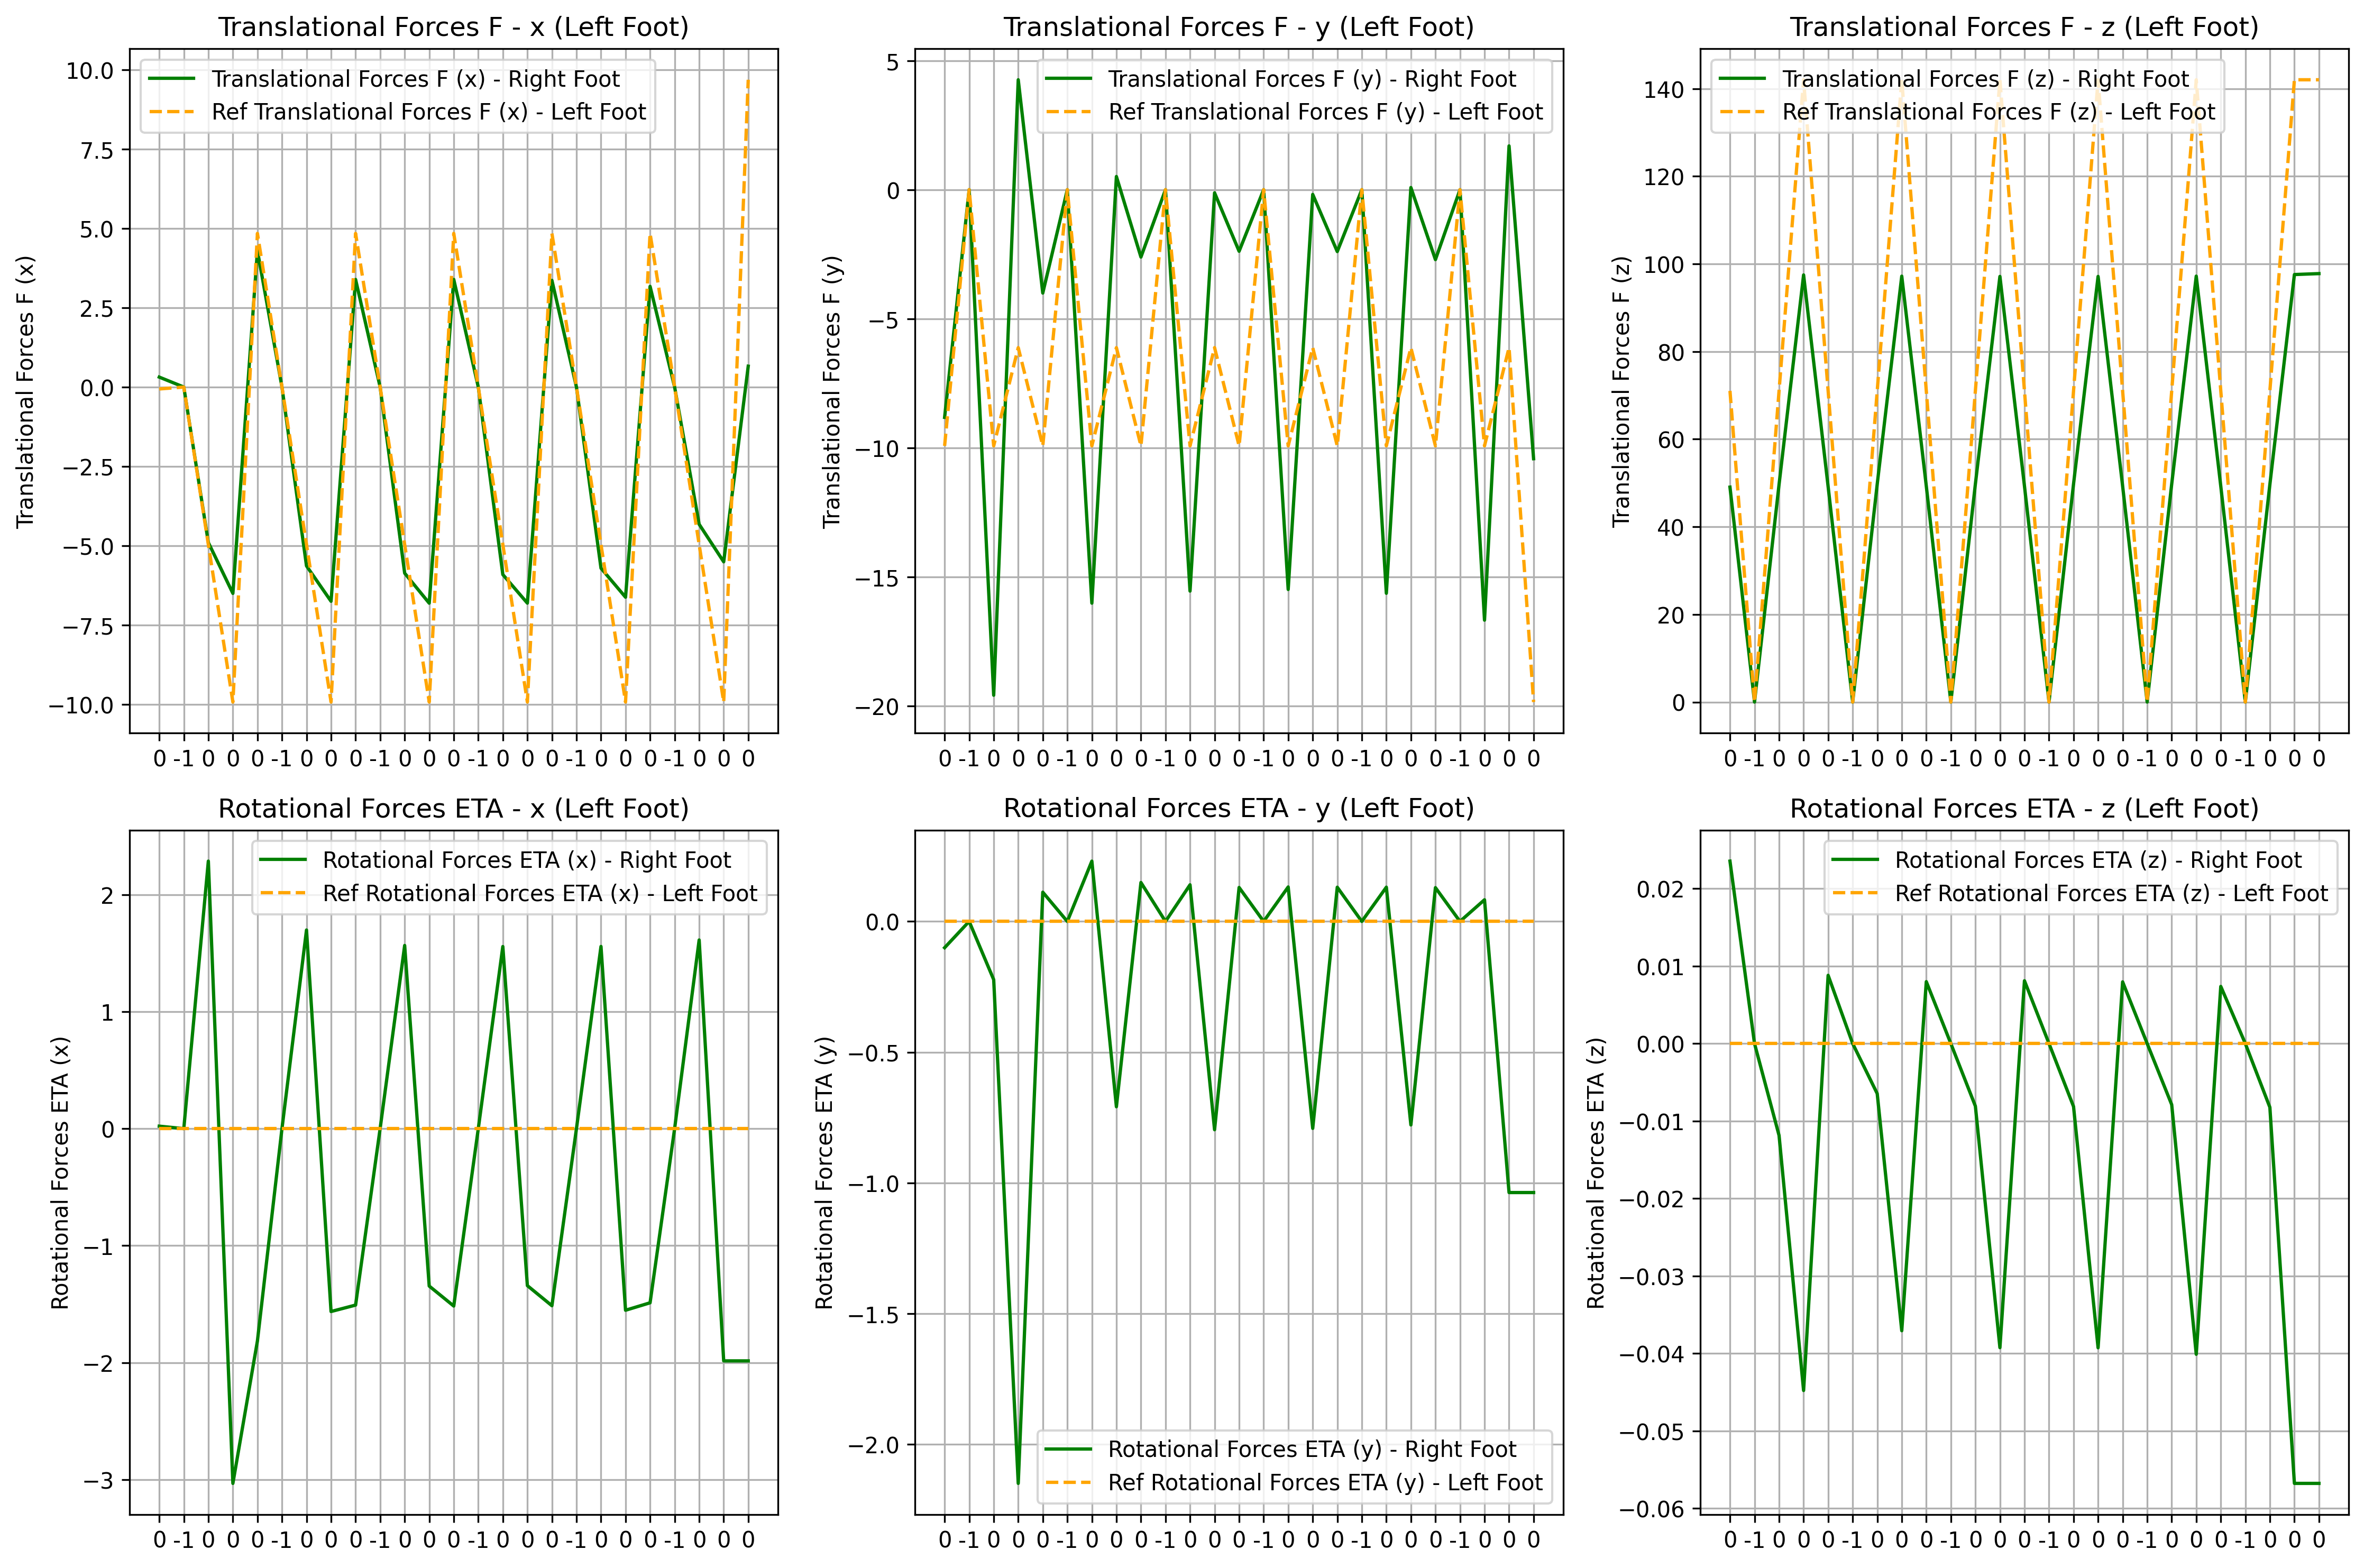
\includegraphics[width=0.8\textwidth]{figures/contact_forces_walking.png}
%     \caption{Trajectory vs Reference: Forces}
%     \label{fig:contact_forces_walking}
% \end{figure}

% \newpage
% \subsubsection{Robot representation}
% In this section it is possible to visualize first the path followed by the CoM, right and left foot in time:
% \begin{figure}[htbp]
%     \centering
%     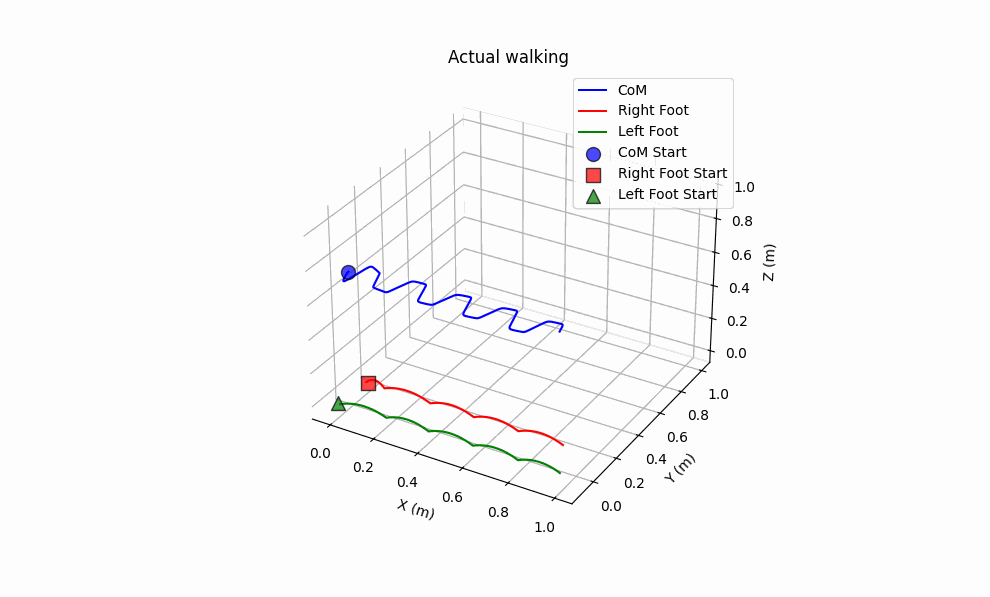
\includegraphics[width=0.8\textwidth]{figures/walking.PNG}
%     \caption{Walking}
%     \label{fig:walking}
% \end{figure}

% The CoM solution and reference foot are also passed to the URDF Skeleton into the Dart Simulation environment. 

% \centering
% \includemedia[
%   width=0.8\linewidth,
%   height=0.45\linewidth,
%   activate=onclick,
%   addresource=figures/walking_sim.mp4,
%   flashvars={
%      source=figures/walking_sim.mp4
%     &autoPlay=true
%   }
% ]{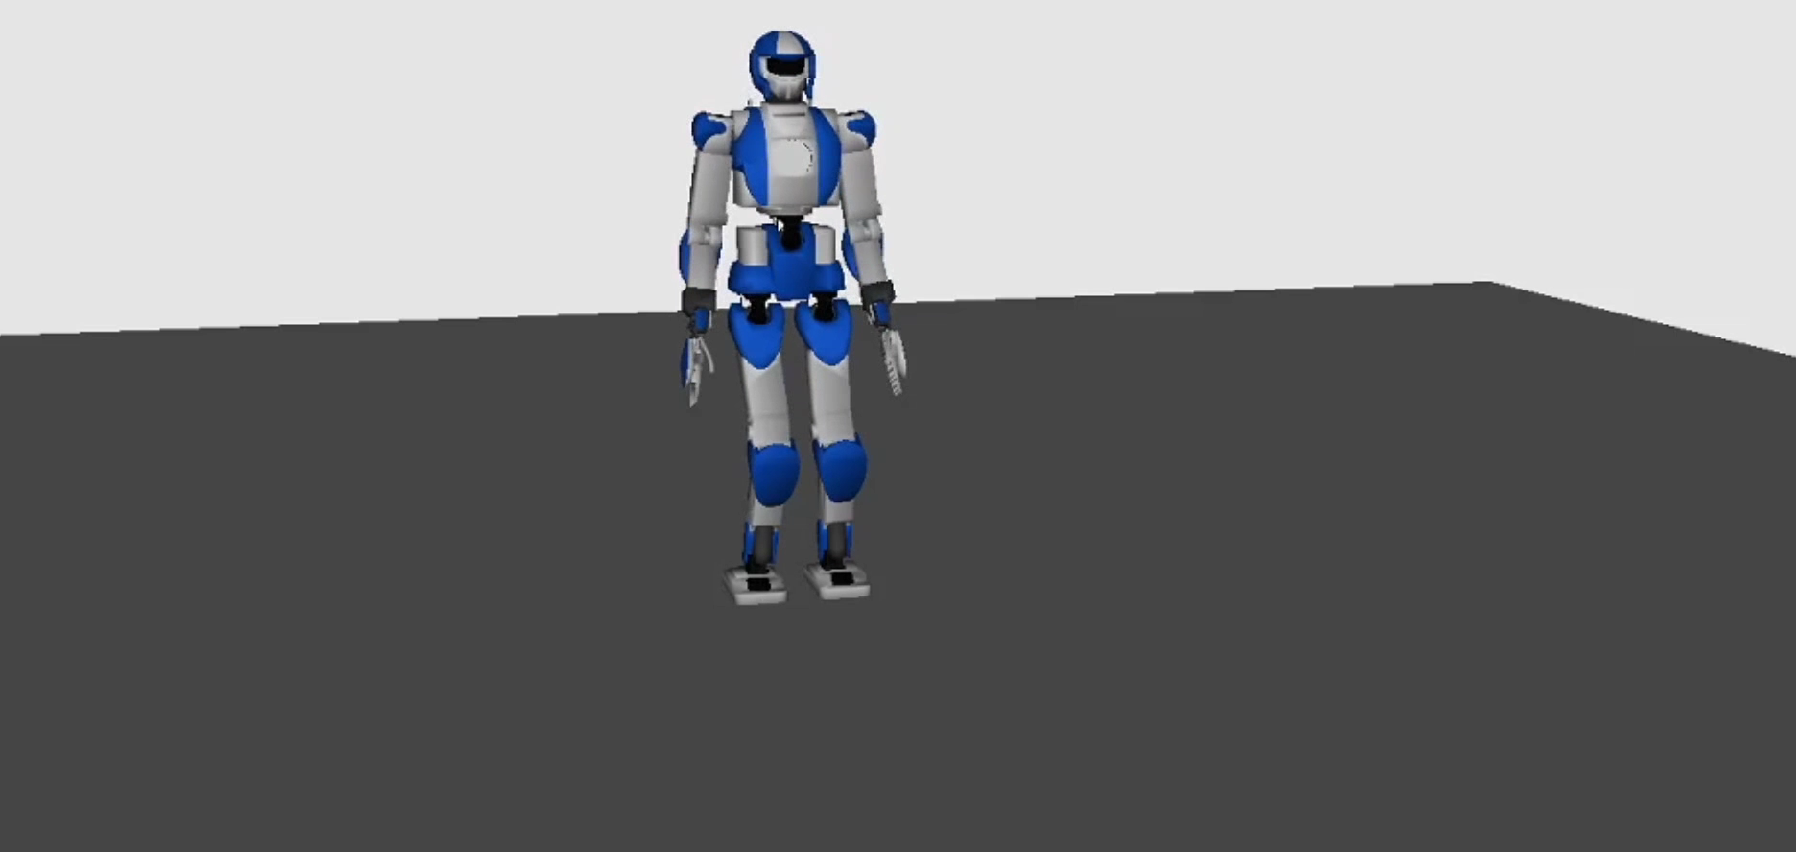
\includegraphics{figures/robot.PNG}}{VPlayer.swf}
 


\end{document}